%definira klasu dokumenta 
\documentclass[12pt]{report} 

%prostor izmedu naredbi \documentclass i \begin{document} se zove uvod. U njemu se nalaze naredbe koje se odnose na cijeli dokument

%osnovni LaTex ne može riješiti sve probleme, pa se koriste različiti paketi koji olakšavaju izradu željenog dokumenta
\usepackage[croatian]{babel} 
\usepackage{amssymb}
\usepackage{amsmath}
\usepackage{txfonts}
\usepackage{mathdots}
\usepackage{titlesec}
\usepackage{array}
\usepackage{lastpage}
\usepackage{etoolbox}
\usepackage{tabularray}
\usepackage{color, colortbl}
\usepackage{adjustbox}
\usepackage{geometry}
\usepackage[classicReIm]{kpfonts}
\usepackage{hyperref}
\usepackage{fancyhdr}

\usepackage{float}
\usepackage{setspace}
\restylefloat{table}


\patchcmd{\chapter}{\thispagestyle{plain}}{\thispagestyle{fancy}}{}{} %redefiniranje stila stranice u paketu fancyhdr

%oblik naslova poglavlja
\titleformat{\chapter}{\normalfont\huge\bfseries}{\thechapter.}{20pt}{\Huge}
\titlespacing{\chapter}{0pt}{0pt}{40pt}


\linespread{1.3} %razmak između redaka

\geometry{a4paper, left=1in, top=1in,}  %oblik stranice

\hypersetup{ colorlinks, citecolor=black, filecolor=black, linkcolor=black,	urlcolor=black }   %izgled poveznice


%prored smanjen između redaka u nabrajanjima i popisima
\newenvironment{packed_enum}{
	\begin{enumerate}
		\setlength{\itemsep}{0pt}
		\setlength{\parskip}{0pt}
		\setlength{\parsep}{0pt}
	}{\end{enumerate}}

\newenvironment{packed_item}{
	\begin{itemize}
		\setlength{\itemsep}{0pt}
		\setlength{\parskip}{0pt}
		\setlength{\parsep}{0pt}
	}{\end{itemize}}




%boja za privatni i udaljeni kljuc u tablicama
\definecolor{LightBlue}{rgb}{0.9,0.9,1}
\definecolor{LightGreen}{rgb}{0.9,1,0.9}

%Promjena teksta za dugačke tablice
\DefTblrTemplate{contfoot-text}{normal}{Nastavljeno na idućoj stranici}
\SetTblrTemplate{contfoot-text}{normal}
\DefTblrTemplate{conthead-text}{normal}{(Nastavljeno)}
\SetTblrTemplate{conthead-text}{normal}
\DefTblrTemplate{middlehead,lasthead}{normal}{Nastavljeno od prethodne stranice}
\SetTblrTemplate{middlehead,lasthead}{normal}

%podesavanje zaglavlja i podnožja

\pagestyle{fancy}
\lhead{Programsko inženjerstvo}
\rhead{$<$Projektni zadatak$>$}
\lfoot{$<$Naziv grupe$>$}
\cfoot{stranica \thepage/\pageref{LastPage}}
\rfoot{\today}
\renewcommand{\headrulewidth}{0.2pt}
\renewcommand{\footrulewidth}{0.2pt}


\begin{document} 
	
	
	
	\begin{titlepage}
		\begin{center}
			\vspace*{\stretch{1.0}} %u kombinaciji s ostalim \vspace naredbama definira razmak između redaka teksta
			\LARGE Programsko inženjerstvo\\
			\large Ak. god. 2023./2024.\\
			
			\vspace*{\stretch{3.0}}
			
			\huge $<$Naziv projekta$>$\\
			\Large Dokumentacija, Rev. \textit{$<$1 ili 2$>$}\\
			
			\vspace*{\stretch{12.0}}
			\normalsize
			Grupa: \textit{$<$Naziv grupe$>$}\\
			Voditelj: \textit{$<$Ime i prezime voditelja$>$}\\
			
			
			\vspace*{\stretch{1.0}}
			Datum predaje: \textit{$<$dan$>$. $<$mjesec$>$. $<$godina$>$.}\\
	
			\vspace*{\stretch{4.0}}
			
			Nastavnik: \textit{$<$Ime i prezime nastavnika zaduženog za vašu grupu$>$}\\
		
		\end{center}

	
	\end{titlepage}

	
	\tableofcontents


	\chapter{Dnevnik promjena dokumentacije}
		
		\textbf{\textit{Kontinuirano osvježavanje}}\\
				
		
		\begin{longtblr}[
				label=none
			]{
				width = \textwidth, 
				colspec={|X[2]|X[13]|X[3]|X[3]|}, 
				rowhead = 1
			}
			\hline
			\textbf{Rev.}	& \textbf{Opis promjene/dodatka} & \textbf{Autori} & \textbf{Datum}\\[3pt] \hline
			0.1 & Napravljen predložak, opis projektnog zadatka i funkcionalni zahtjevi & Daniel Rodić, Lovro Petrović & 1.11.2023. \\[3pt] \hline 
			0.2 & Arhitektura i dizajn sustava.& Nina \newline Kolobarić, Daniel Rodić & 8.11.2023.\\[3pt] \hline 
			0.3 & Dodani obrazci uporabe &Vedran Lugarić, Daniel Rodić & 8.11.2023. \\[3pt] \hline 
			0.4 & Dodani UML i sekvencijski dijagrami & Lovro Petrović, Lukas Schönberger, Daniel Rodić & 13.11.2023. \\[3pt] \hline
			0.5 & U poglavlju Specifikacija programske potpore ažuriran aktor Autor te ispravljeni nepotrebni znakovi &Daniel Rodić & 13.11.2023. \\[3pt] \hline 
			0.6 & Ispravljen tekst koji je bio u kurzivu a nije trebao biti &Daniel Rodić & 13.11.2023. \\[3pt] \hline 
			0.7 & Dodan opis baze podataka, opis tablica baze podataka te dijagram baze podataka &Domagoj Žokalj, Josip Maradin, Daniel Rodić & 15.11.2023. \\[3pt] \hline 
            0.8 & Dodana popravljena baza podataka sa opisom i dijagramom baze podataka &Vedran Lugarić & 15.11.2023. \\[3pt] \hline
            0.9 & Dodan frontend &Lukas Schönberger & 15.11.2023. \\[3pt] \hline
            1.0 & Preuređen cijeli frontend u Reactu & Nina \newline Kolobarić & 9.12.2023. \\[3pt] \hline
            1.1 & Na frontednu dodana registracija & Nina \newline Kolobarić & 11.12.2023. \\[3pt] \hline
            1.2 & Izrada i update backenda u djangu te update frontedna  & Lukas Schönberger, Lovro Petrović & 11.12.2023. \\[3pt] \hline
            1.3 & Update backenda, dovršena registracija  & Lukas Schönberger, Lovro Petrović & 12.12.2023. \\[3pt] \hline
            1.4 & Omogućena prijava i odjava te stranice samo za prijavljene korisnike  & Lukas Schönberger & 13.12.2023. \\[3pt] \hline
            1.5 & Dodana stranica za prikaz konferencija u forntendu & Nina Kolobarić & 14.12.2023. \\[3pt] \hline
            1.6 & Dodavanje lozinke kod prijave te hashiranje i spremanje iste u bazu & Lukas Schönberger, Lovro Petrović & 17.12.2023. \\[3pt] \hline
            1.7 & Backend prebacen u flask te dodana prijava i odjava  & Lukas Schönberger, Lovro Petrović & 18.12.2023. \\[3pt] \hline
            1.8 & Napravljene izmjene i dodana stranica za prikaz postera u forntendu & Lukas Schönberger, Nina Kolobarić & 18.12.2023. \\[3pt] \hline
            1.9 & Dodano dimaničko učitavanje konferencija i dodana baza podataka  & Lukas Schönberger, Lovro Petrović, Daniel Rodić, Vedran Lugarić, Josip Maradin, Domagoj Žokalj & 19.12.2023. \\[3pt] \hline
            1.10 & Popravljeno dinamičko prikazivanje konferencija i u frontendu dodano dodavanje konferencija i postera & Lukas Schönberger, Nina Kolobarić & 20.12.2023. \\[3pt] \hline
            1.11 & Provjera lozinke za pristup konferenciji u backendu & Lovro Petrović & 27.12.2023. \\[3pt] \hline
            1.12 & Dodane rute za pristup radovima u bazi, napravljena struktura na backendu & Lukas Schönberger, Domagoj Žokalj, Lovro Petrović, Vedran Lugarić & 28.12.2023. \\[3pt] \hline
            1.13 & Napravljene i omogućene uloge te manje promjene u frontendu & Lukas Schönberger, Lovro Petrović, Vedran Lugarić & 29.12.2023. \\[3pt] \hline
            1.14 & Dinamički ispis radova & Lukas Schönberger, Domagoj Žokalj & 31.12.2023. \\[3pt] \hline
            1.15 & Popup za lozinku za konferenciju dodan & Nina Kolobarić & 5.1.2024. \\[3pt] \hline
            1.16 & Omogućeno dodavanje postera i konferencija unutar aplikacije  & Lukas Schönberger, Lovro Petrović & 6.1.2024. \\[3pt] \hline
            1.17 & Uređeno sučelje za dodavanje radova te omogućeno glasanje i prikazivanje postera  & Lukas Schönberger, Lovro Petrović, Nina Kolobarić, Vedran Lugarić & 7.1.2024. \\[3pt] \hline
            1.18 & Uređivanje projekta  & Lukas Schönberger, Lovro Petrović, Nina Kolobarić, Daniel Rodić, Vedran Lugarić & 8.1.2024. \\[3pt] \hline
            1.19 & Popravljen logout, uljepšan frontend te iplementiran weather app  & Lukas Schönberger, Nina Kolobarić, Vedran Lugarić, Daniel Rodić & 9.1.2024. \\[3pt] \hline
            1.20 & Preuređen weather app, deployana baza podataka, dodano automatsko slanje e-maila po završetku konferenicije & Lukas Schönberger, Lovro Petrović, Nina Kolobarić, Vedran Lugarić & 10.1.2024. \\[3pt] \hline
            1.21 & Uljepšan forntend, omogućen upload ppt i pdf te dodano prikazivanje pokrovitelja  & Lukas Schönberger, Lovro Petrović, Nina kolobarić& 11.1.2024. \\[3pt] \hline
            1.22 & Popravljena baza podataka, prepavljena aplikacija prema novoj bazi, dodana galerija, omogućeno dobijanje radova od strane voditelja i administratora, omogućen download radova i popravljen frontend  & Lukas Schönberger, Lovro Petrović, Nina Kolobarić, Vedran Lugarić & 12.1.2024. \\[3pt] \hline
            1.23 & Dodana poruka obavijesti za neuspjelu registraciju i login  & Lukas Schönberger, Domagoj Žokalj & 13.1.2024. \\[3pt] \hline
            1.24 & Dodana verifikacija mail adrese, promjenje uloga i dodan responzivni dizajn za konferencije, stranice dodavanja i prošle konferencije  & Lukas Schönberger, Lovro Petrović, Nina Kolobarić & 14.1.2024. \\[3pt] \hline
            1.25 & Uređeni pokrovitelji te pistup live prijenosu i galerija  & Lukas Schönberger, Lovro Petrović, Nina KOlobarić, Daniel Rodić, Vedran Lugarić & 15.1.2024. \\[3pt] \hline

			&  &  & \\[3pt] \hline	
		\end{longtblr}
	
	

	\chapter{Opis projektnog zadatka}
		
		Svrha ovog projekta je razvoj programske potpore za web aplikaciju "Digitalni poster" koja će se koristiti u svrhe održavanja stručnih konferencija. Aplikacija će omogućiti pregled radova sudionika i dati im mogućnosti ocjenjivanja pojedinog rada. Svaki stručni rad bit će prikazan u obliku postera, koji se sastoji od stručnog rada i/ili izlaganja autora, te će autori moći dodati odgovarajuću prezentaciju za svoj rad. Svi će događaji biti fotografirani, a odabrane fotografije će tijekom konferencije biti dostupne svim registriranim korisnicima.

		Prilikom prvog pokretanja aplikacije prikazuje se...

		Za registraciju potrebni su sljedeći podaci:

		\begin{packed_item}
			\item {ime i prezime}
			\item {e-mail adresa}
			\item {lozinka}
			\item {broj mobitela}
		\end{packed_item}
		Prilikom registracije u sustav korisniku se automatski dodjeljuje status posjetitelja te mu se naknadno može dodijeliti status autora, voditelja ili administratora. Svaki registrirani korisnik može pristupiti svojim osobnim podacima koje može mijenjati te može obrisati svoj račun.

		\textbf{\underline{Posjetitelj}} konferencije ima minimalna prava u samoj aplikaciji, to jest posjetitelj može pregledati termine konferencija, mjesto konferencija te vremenske prilike u mjestu konferencije. U terminu konferencije posjetitelj može pristupiti samoj konferenciji prijavom za istu. Nakon prijave u konferenciju posjetitelju je dostupno direktno video praćenje trenutnih događanja u glavnoj konferencijskoj dvorani te su mu dostupni promotivni materijali pokrovitelja konferencije. Također posjetitelju je dodijeljeno pravo glasa za točno jedan poster koji predstavlja pojedinog autora. Glasovanje je moguće samo tijekom određenog razdoblja, odnosno u terminu održavanja konferencije. Kada završi sam postupak glasovanja posjetitelju kao i svim registriranim korisnicima dostupni su rezultati glasovanja. Posjetitelja će se elektroničkom poštom obavijestiti o mjestu i vremenu održavanja dodjele nagrada za prva tri mjesta. Sve dostupne fotografije s konferencije posjetitelj će moći spremati lokalno na svoj uređaj.

		\textbf{\underline{Autor}} ima slična prava kao posjetitelj. Razlikuju se po tome što autor ne može glasati kako bi se izbjegli konflikti i subjektivnost. Autor sve potrebne materijale šalje voditelju putem elektroničke pošte. Autori nakon završetka glasanja dobivaju obavijest o svom rangu, a autori prva tri rangirana rada dobivaju pozivnicu za dodjelu nagrada.

		\textbf{\underline{Voditelj}} konferencije vrši prijavu autora, radova i postera za svoju konferenciju te su mu dostupni svi podaci istih. Također voditelj mora organizirati konferenciju tako da rezervira dvorane te od administratora traži unos svih podataka, datum, vrijeme i mjesto, u aplikaciju. Odabrane fotografije dostupne svim korisnicima za spremanje lokalno na uređaj ovjerene su od strane voditelja. Voditelj nakon glasanja sastavlja rang listu koju šalje adminu koji ju čini dostupnom svim korisnicima te obavijesti svakog autora o njegovom rangu. Dodjela nagrada za prva tri mjesta također je organizirana od strane voditelja koji osigurava novčane nagrade za svakog od pobjednika ovisno o samom rangu autora. Također mora rezervirati dvoranu za isti događaj.

		\textbf{\underline{Administrator}} sustava ima najveće ovlasti te definira sve uvjete za ispravan rad sustava. Dostupni su mu svi podaci svakog registriranog korisnika kojima može promijeniti ovlasti ili im obrisati račun. Admin odobrava i vrši zahtjeve koje dobije od voditelja. Zadužen je za konstantno ažuriranje kalendara događaja te mora paziti da ne dođe do konflikata, odnosno da se dvije konferencije ne održavaju u isto vrijeme na istom mjestu. Uz to admin može obrisati svaki prijavljeni poster koji nije primjeren iz bilo kojeg razloga.
		

				

		
	
	\chapter{Specifikacija programske potpore}
		
	\section{Funkcionalni zahtjevi}
			
			\noindent \textbf{Dionici:}
			
			\begin{packed_enum}
				
				\item Administrator
				\item Voditelj			
				\item Posjetitelj
				\item Razvojni tim
				
			\end{packed_enum}
			
			\noindent \textbf{Aktori i njihovi funkcionalni zahtjevi:}
			
			
			\begin{packed_enum}
				\item  \underbar{Neregistrirani korisnik (inicijator) može:}
				
				\begin{packed_enum}
					
					\item stvoriti novi račun registracijom za koju su mu potrebni ime i prezime, e-mail, korisničko ime, lozinka
					\item pregledati kalendar događaja, odnosno može vidjeti:
					\begin{packed_enum}
						
						\item  vrijeme konferencije
						\item  mjesto konferencije
						\item  aktivne i nadolazeće konferencije
				
					\end{packed_enum}
					
				\end{packed_enum}

				\item  \underbar{Posjetitelj (inicijator) može:}
				
				\begin{packed_enum}
					
					\item pokrenuti direktno video praćenje događaja neke konferencije
					\item glasati za točno jedan poster
					\item spremati fotografije lokalno na svoj uređaj
					\item dodavati postere u nadolazeće konferencije

				\end{packed_enum}


				\item  \underbar{Administrator (inicijator) može:}
				
				\begin{packed_enum}
					
					\item dodati konferenciju s kalendara
					\item dodati i/ili izbrisati poster
					\item dodati ulogu voditelja nekon registriranom korisniku za određenu konferenciju
					
				\end{packed_enum}

			
				\item  \underbar{Baza podataka (sudionik):}
				
				\begin{packed_enum}
					
					\item sadrži podatke o svim korisnicima i njihovom statusu
					\item sadrži podatke o svim održanim ili budućim konferencijama
					\item sadrži podatke o svakom posteru, autoru, broju glasova, krajnjem rangu i ulogama
					\item sadrži podatke o pokroviteljima konferencije i reklamama
					
				\end{packed_enum}
			\end{packed_enum}
			
			\eject 
			
			
				
			\subsection{Obrasci uporabe}
				
				\subsubsection{Opis obrazaca uporabe}
					
					\noindent \underbar{\textbf{UC1 -Registracija}}
					\begin{packed_item}
	
						\item \textbf{Glavni sudionik: }Autor, posjetitelj
						\item  \textbf{Cilj:} stvoriti korisnički račun za prijavu u sustav
						\item  \textbf{Sudionici:} Baza podataka
						\item  \textbf{Preduvjet:} -
						\item  \textbf{Opis osnovnog tijeka:}
						
						\item[] \begin{packed_enum}
	
							\item Korisnik odabere opciju za registraciju
							\item Unosi potrebne korisničke podatke
							\item Obavještava ga se o uspješno registracijii
						\end{packed_enum}
						
						\item  \textbf{Opis mogućih odstupanja:}
						
						\item[] \begin{packed_item}
	
							\item Unos postojećeg ili nezadovoljavajuće e-maila

							\item[] \begin{packed_enum}
								
								\item Obavještavanje korisnika o neuspjeloj registraciji
								\item Vraćanje korisnika na početak tj. ponovnu registracij
								\item Korisnik mijenja podatke ili odustaje od registracije
								
							\end{packed_enum}
							
						\end{packed_item}
					\end{packed_item}

					\noindent \underbar{\textbf{UC2 -Pregled konferencija}}
					\begin{packed_item}
	
						\item \textbf{Glavni sudionik: }Autor, posjetitelj
						\item  \textbf{Cilj:} Pregled konferencija
						\item  \textbf{Sudionici:} Baza podataka
						\item  \textbf{Preduvjet:} -
						\item  \textbf{Opis osnovnog tijeka:}
						
						\item[] \begin{packed_enum}
	
							\item Sve dostupne konferencije su prikazane prilikom otvaranja aplikacije
							\item Korisnik odabire konferenciju koji hoće
							\item Prije nego mu se dopusti pristup konferenciji korisnik treba biti registriran
						\end{packed_enum}
						
					\end{packed_item}

					\noindent \underbar{\textbf{UC3 -Pregled radova}}
					\begin{packed_item}
	
						\item \textbf{Glavni sudionik: }Autor, posjetitelj
						\item  \textbf{Cilj:} Pregled konferencija
						\item  \textbf{Sudionici:} Baza podataka
						\item  \textbf{Preduvjet:} Registracija u sustav, prijavljen u konferenciju
						\item  \textbf{Opis osnovnog tijeka:}
						
						\item[] \begin{packed_enum}
	
							\item Ulazak na neku određenu konferenciju
							\item Prikaz svih radova 
						\end{packed_enum}
						
					\end{packed_item}

					\noindent \underbar{\textbf{UC4 -Ocjenjivanje radova}}
					\begin{packed_item}
	
						\item \textbf{Glavni sudionik: }Posjetitelj
						\item  \textbf{Cilj:} Davanje svog glasa jednom od radova
						\item  \textbf{Sudionici:} Baza podataka, posjetitelj
						\item  \textbf{Preduvjet:} Uspješna prijava u konferenciju
						\item  \textbf{Opis osnovnog tijeka:}
						
						\item[] \begin{packed_enum}
	
							\item Odabir rada kojem se odlučuje dati glas 
							\item Davanje glasa odabranom radu
						\end{packed_enum}
						
					\end{packed_item}

					\noindent \underbar{\textbf{UC5 -Prijava u konferenciju}}
					\begin{packed_item}
	
						\item \textbf{Glavni sudionik: }Autor, posjetitelj
						\item  \textbf{Cilj:} Prijava u konferenciju radi pregleda radova
						\item  \textbf{Sudionici:} Baza podataka
						\item  \textbf{Preduvjet:} Registracija korisnik
						\item  \textbf{Opis osnovnog tijeka:}
						
						\item[] \begin{packed_enum}
	
							\item Odabir određene konferencije za koju želite pristup
							\item Upisivanje lozinke za tu konferenciju uz uvjet da ste prijavljeni
							\item Dobivanje pristupa konferenciji
						\end{packed_enum}
						
					\end{packed_item}

					\noindent \underbar{\textbf{UC6 -Otvaranje nove konferencije}}
					\begin{packed_item}
	
						\item \textbf{Glavni sudionik: }Administrator
						\item  \textbf{Cilj:} Otvaranje konferencije
						\item  \textbf{Sudionici:} Baza podataka, Administrator, Voditelj
						\item  \textbf{Preduvjet:} Odobrenje administratora
						\item  \textbf{Opis osnovnog tijeka:}
						
						\item[] \begin{packed_enum}
	
							\item Kontaktiranje administratora radi otvaranja nove konferencije
							\item Otvaranje konferencije od strane administratora te dodjeljivanje voditelja
						\end{packed_enum}
						
					\end{packed_item}

					\noindent \underbar{\textbf{UC7 -Pregled vremenske prognoze}}
					\begin{packed_item}
	
						\item \textbf{Glavni sudionik: }Autor, posjetitelj
						\item  \textbf{Cilj:} Pregled vremenske prognoze za određenu konferenciju
						\item  \textbf{Sudionici:} Baza podataka
						\item  \textbf{Preduvjet:} Registracija korisnika, odabir konferencije
						\item  \textbf{Opis osnovnog tijeka:}
						
						\item[] \begin{packed_enum}
	
							\item Nakon odabrane konferencije na dnu stranice će biti moguće vidjeti vremensku prognozu za lokaciju te konferencije$>$
						\end{packed_enum}
						
					\end{packed_item}

					\noindent \underbar{\textbf{UC8-Dodavanje rada u konferenciju}}
					\begin{packed_item}
	
						\item \textbf{Glavni sudionik: }Autor, voditelj
						\item  \textbf{Cilj:} Dodavanje/prijava rada na nekoj konferenciji
						\item  \textbf{Sudionici:} Baza podataka, Voditelj, Autor
						\item  \textbf{Preduvjet:} -
						\item  \textbf{Opis osnovnog tijeka:}
						
						\item[] \begin{packed_enum}
	
							\item Autor šalje mail s radom voditelju konferencije
							\item Voditelj konferencije dodaje rad u konferenciju kako bi se mogao prikazati
						\end{packed_enum}
						
					\end{packed_item}

					\noindent \underbar{\textbf{UC9-Video praćenje konferencije}}
					\begin{packed_item}
	
						\item \textbf{Glavni sudionik: }Posjetitelj
						\item  \textbf{Cilj:} Praćenje konferencije online
						\item  \textbf{Sudionici:} Baza podataka, posjetitelj
						\item  \textbf{Preduvjet:} Registracija korisnika
						\item  \textbf{Opis osnovnog tijeka:}
						
						\item[] \begin{packed_enum}
	
							\item Korisnik se mora registrirati
							\item Nakon što je korisnik registriran može odabrati online praćenje
						\end{packed_enum}
						
					\end{packed_item}

					\noindent \underbar{\textbf{UC10 -Login}}
					\begin{packed_item}
	
						\item \textbf{Glavni sudionik: }Neprijavljeni korisnik
						\item  \textbf{Cilj:} prijava u već postojeći korisnički račun
						\item  \textbf{Sudionici:} Baza podataka
						\item  \textbf{Preduvjet:} Postojeći korisnički račun
						\item  \textbf{Opis osnovnog tijeka:}
						
						\item[] \begin{packed_enum}
	
							\item Korisnik odabere opciju za login
							\item Unosi potrebne korisničke podatke
							\item potvrđuje da nije robot
							\item pritišće gumb login
						\end{packed_enum}
						
						\item  \textbf{Opis mogućih odstupanja:}
						
						\item[] \begin{packed_item}
	
							\item Unos nepostojećeg ili nezadovoljavajuće e-maila
							\item Unos pogrešne lozinke
							\item Polje potvrde da nije robot je prazno

							\item[] \begin{packed_enum}
								
								\item Obavještavanje korisnika o neuspjeloj login-u
								\item Korisnik mijenja podatke ili odustaje od login-a
								
							\end{packed_enum}
							
						\end{packed_item}
					\end{packed_item}

					\noindent \underbar{\textbf{UC11 -Logout}}
					\begin{packed_item}
	
						\item \textbf{Glavni sudionik: }Autor, posjetitelj
						\item  \textbf{Cilj:} odjava iz sustava
						\item  \textbf{Sudionici:} Baza podataka
						\item  \textbf{Preduvjet:} Prethodno je potrebno biti prijavljen u sustav
						\item  \textbf{Opis osnovnog tijeka:}
						
						\item[] \begin{packed_enum}
	
							\item Korisnik odabire opciju za odjavu
							
						\end{packed_enum}
						
					\end{packed_item}

					\noindent \underbar{\textbf{UC12 -Odabir postera}}
					\begin{packed_item}
	
						\item \textbf{Glavni sudionik: }Voditelj
						\item  \textbf{Cilj:} odabir postera za prikaz na konferenciji
						\item  \textbf{Sudionici:} Baza podataka
						\item  \textbf{Preduvjet:} Imati administratorka dopustenja te biti prijavljen u sustav
						\item  \textbf{Opis osnovnog tijeka:}
						
						\item[] \begin{packed_enum}
	
							\item Administrator odabire opciju dodavanje potsera te ide na "Pregledaj unesene radove"
							\item Odabire radove koji se mogu prikazati na konferenciji
						\end{packed_enum}
						
						
					\end{packed_item}

					\noindent \underbar{\textbf{UC13 -Pregled PDF-a}}
					\begin{packed_item}
	
						\item \textbf{Glavni sudionik: }Voditelj, posjetitelj, administrator
						\item  \textbf{Cilj:} Pogledati PDF nekog postera na konferenciji
						\item  \textbf{Sudionici:} Baza podataka
						\item  \textbf{Preduvjet:} Obavljen login i omogućen pristup konferenciji
						\item  \textbf{Opis osnovnog tijeka:}
						
						\item[] \begin{packed_enum}
	
							\item Korisnik pristupa konferenciji
							\item Kod postera čiji pdf želi vidjeti pritišće gumb "pdf"
							\item Otvara se pdf postera
						\end{packed_enum}
						
					\end{packed_item}

					\noindent \underbar{\textbf{UC14 -Preuzimanje ppt-a}}
					\begin{packed_item}
	
						\item \textbf{Glavni sudionik: }Voditelj, posjetitelj, administrator
						\item  \textbf{Cilj:} Preuzimanje ppta-a nekog postera na konferenciji lokalno
						\item  \textbf{Sudionici:} Baza podataka
						\item  \textbf{Preduvjet:} Obavljen login i omogućen pristup konferenciji
						\item  \textbf{Opis osnovnog tijeka:}
						
						\item[] \begin{packed_enum}
	
							\item Korisnik pristupa konferenciji
							\item Kod postera čiji ppt želi preuzeti pritišće gumb "ppt"
							\item Preuzima se ppt
						\end{packed_enum}
						
					\end{packed_item}

					\noindent \underbar{\textbf{UC15 -Dodavanje voditelja}}
					\begin{packed_item}
	
						\item \textbf{Glavni sudionik: }Administrator
						\item  \textbf{Cilj:} Dodavanje uloge voditelja nekom registriranom korisniku za određenu konferenciju
						\item  \textbf{Sudionici:} Baza podataka, registrirani korisnik
						\item  \textbf{Preduvjet:} Obavljen login kao administrator 
						\item  \textbf{Opis osnovnog tijeka:}
						
						\item[] \begin{packed_enum}
	
							\item Administrator pristupa nadolazećim konferencijama
							\item Kod konferencije kojoj želi dodati voditelja pritišće gumb "Dodaj voditelja"
							\item upisuje e-mail racuna korisnika kojeg želi postaviti kao voditelja te konferencije
						\end{packed_enum}
						
					\end{packed_item}

					\noindent \underbar{\textbf{UC16 -Dodavanje pokrovitelja}}
					\begin{packed_item}
	
						\item \textbf{Glavni sudionik: }Voditelj, administrator
						\item  \textbf{Cilj:} Dodavanje pokrovitelja za neku konferenciju
						\item  \textbf{Sudionici:} Baza podataka
						\item  \textbf{Preduvjet:} Administratorske ili voditeljske ovlasi 
						\item  \textbf{Opis osnovnog tijeka:}
						
						\item[] \begin{packed_enum}
	
							\item Korisnik pristupa konferenciji
							\item Unutar konferenije pritišće gumb "Dodaj pokrovitelja"
							\item Nakon unesenih potrebnih podataka pritišće gzmb "Unesi" čime je dodan pokrovitelj u konferenciju
						\end{packed_enum}
						
					\end{packed_item}

					\noindent \underbar{\textbf{UC17 -Pregled galerije}}
					\begin{packed_item}
	
						\item \textbf{Glavni sudionik: }Posjetitelj
						\item  \textbf{Cilj:} Pregled slika fotografiranih na konferenciji
						\item  \textbf{Sudionici:} Baza podataka
						\item  \textbf{Preduvjet:} - 
						\item  \textbf{Opis osnovnog tijeka:}
						
						\item[] \begin{packed_enum}
	
							\item Korisnik pristupa proslim konferencijma
							\item Pritišće gumb "Galerija"
							\item Omogućen mu je pregled svih fotografija fotografiranih na toj konferenciji
						\end{packed_enum}
						
					\end{packed_item}

					\noindent \underbar{\textbf{UC18 -Preuzimanje forografija iz galerije}}
					\begin{packed_item}
	
						\item \textbf{Glavni sudionik: }Posjetitelj, baza podataka
						\item  \textbf{Cilj:} Spremanje fotografija lokalno na uređaj
						\item  \textbf{Sudionici:} Baza podataka
						\item  \textbf{Preduvjet:} - 
						\item  \textbf{Opis osnovnog tijeka:}
						
						\item[] \begin{packed_enum}
	
							\item Korisnik pristupa proslim konferencijma
							\item Pritišće gumb "Galerija"
							\item Omogućen mu je pregled svih fotografija fotografiranih na toj konferenciji te može označiti fotogracije koje želi preuzeti ili preuzimati jednu po jednu fotografiju
						\end{packed_enum}
						
					\end{packed_item}
				
				
					
				\subsubsection{Dijagrami obrazaca uporabe}
					
		\begin{figure}[H]
			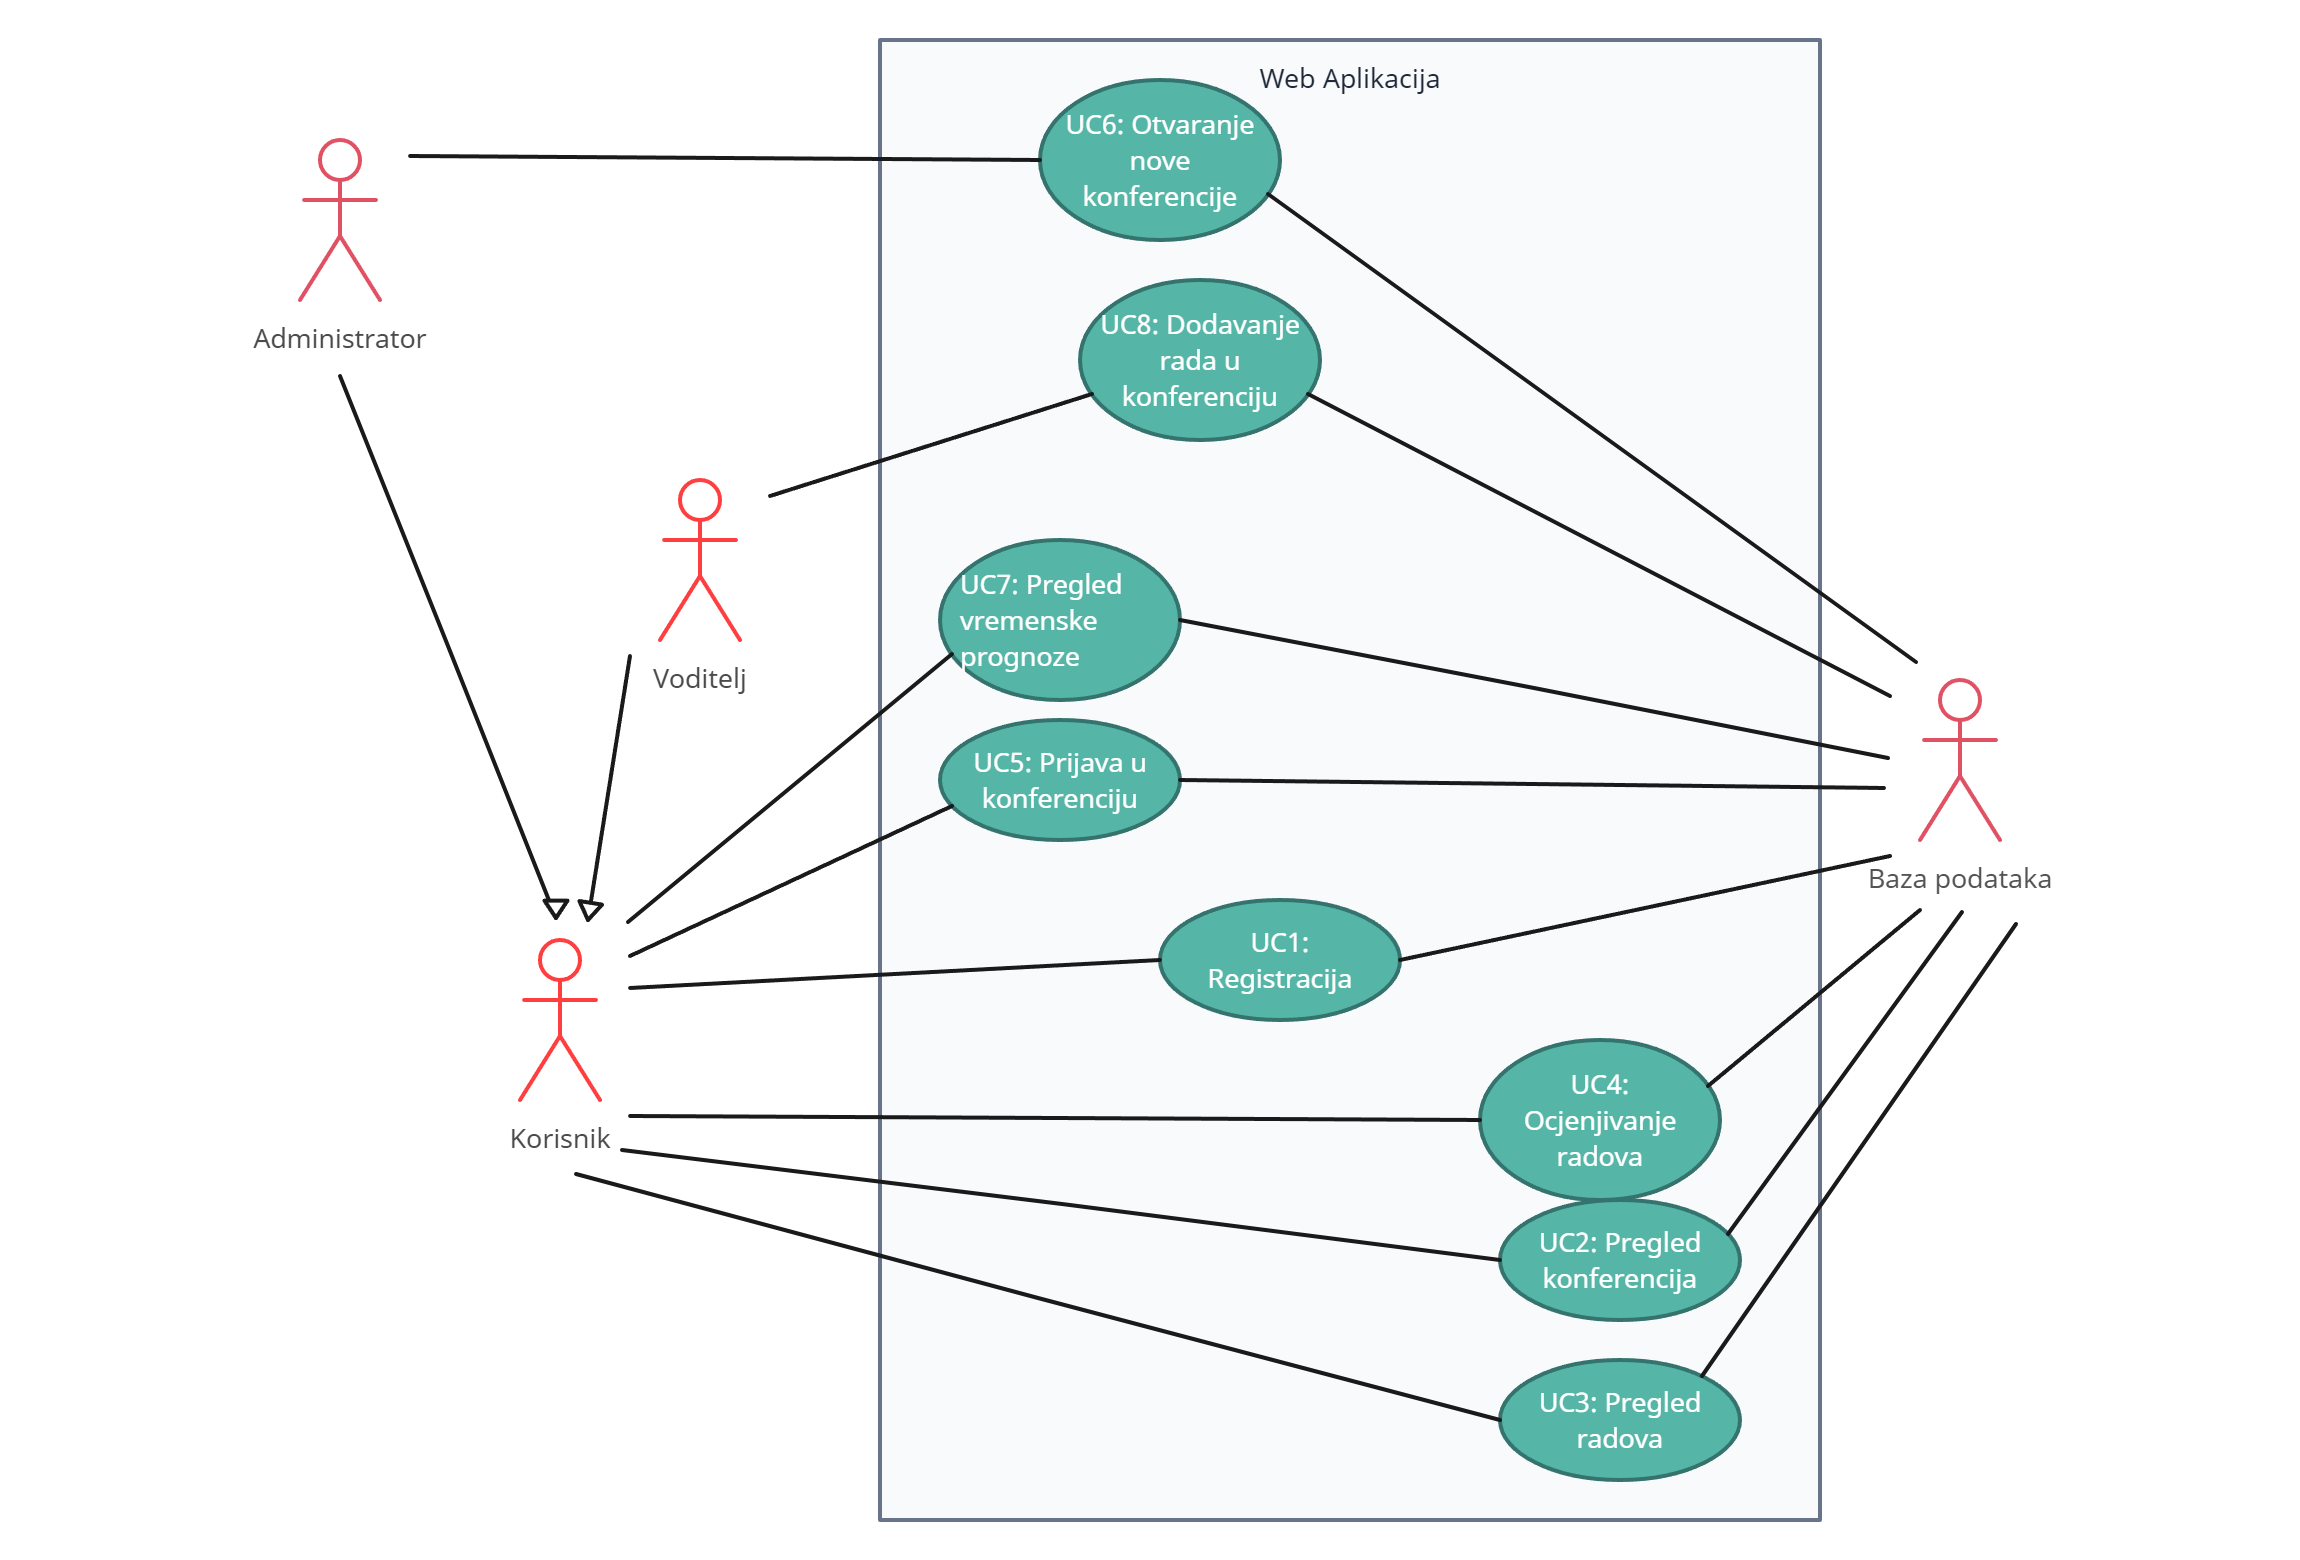
\includegraphics[scale=0.55]{slike/UML1.JPG} 
			\centering
			\caption{Slika 3.1: }
			\label{UML1}
		\end{figure}		
				
			\subsection{Sekvencijski dijagrami}
				
		\begin{figure}[H]
			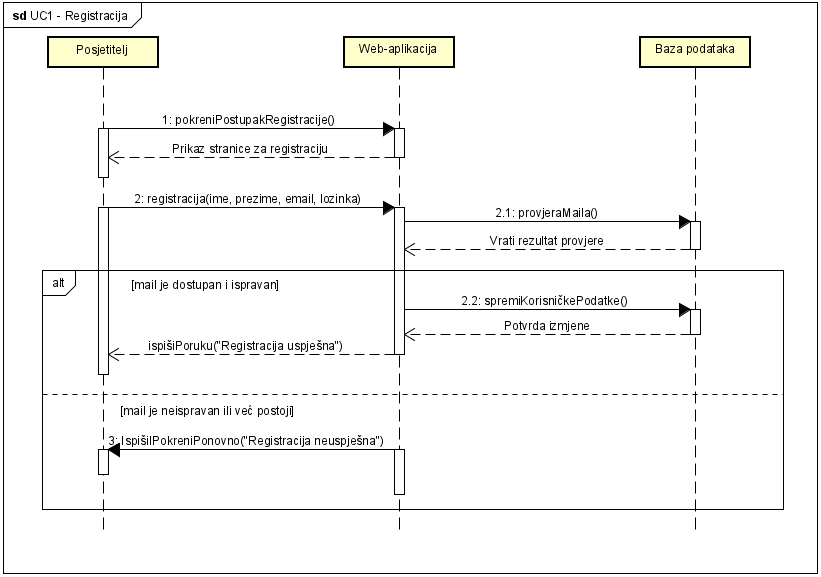
\includegraphics[scale=0.7]{slike/UC1.PNG} 
			\centering
			\caption{Slika 3.2: Sekvencijski dijagram za UC1}
			\label{fig:UC1}
		\end{figure}	

		\begin{figure}[H]
			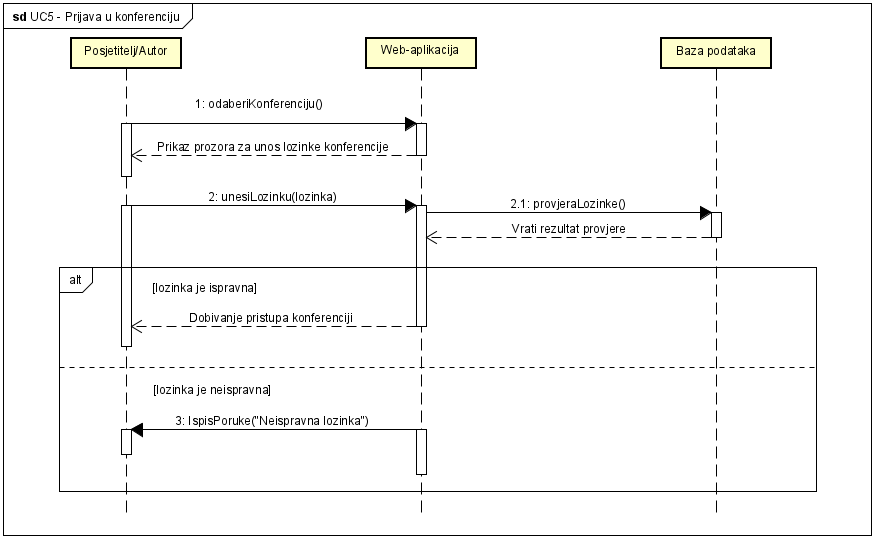
\includegraphics[scale=0.7]{slike/UC5.PNG} 
			\centering
			\caption{Slika 3.3: Sekvencijski dijagram za UC5}
			\label{fig:UC5}
		\end{figure}	
	
		\section{Ostali zahtjevi}
		
			\textbf{\textit{dio 1. revizije}}\\
		 
			 \textit{Nefunkcionalni zahtjevi i zahtjevi domene primjene dopunjuju funkcionalne zahtjeve. Oni opisuju \textbf{kako se sustav treba ponašati} i koja \textbf{ograničenja} treba poštivati (performanse, korisničko iskustvo, pouzdanost, standardi kvalitete, sigurnost...). Primjeri takvih zahtjeva u Vašem projektu mogu biti: podržani jezici korisničkog sučelja, vrijeme odziva, najveći mogući podržani broj korisnika, podržane web/mobilne platforme, razina zaštite (protokoli komunikacije, kriptiranje...)... Svaki takav zahtjev potrebno je navesti u jednoj ili dvije rečenice.}
			 
			 
			 
	
	\chapter{Arhitektura i dizajn sustava}
		
		\textbf{\textit{dio 1. revizije}}\\

		\textit{ Arhitektura sustava ima hijerarhijsku strukturu u kojoj svaki sloj komunicira isključivo s neposredno susjednim slojevima. Naš sustav sastoji se od pet glavnih slojeva: Korisničko sučelje, Kontroler, Servis, Repozitorij i Baza podataka. Korisničko sučelje, ili User Interface (UI) omogućava interakciju između korisnika i računala. Korisničko sučelje našeg sustava razvijeno je uz pomoć Reacta, JavaScript biblioteke koja olakšava stvaranje korisničkih sučelja. Korisničko sučelje šalje zahtjeve kontroleru temeljem korisničkih akcija i koristi JSON (JavaScript Object Notation) datoteke za prijenos podataka. Kontroler, koristeći REST API (Representational State Transfer), upravlja zahtjevima vanjskih korisnika i odgovara na njih. U većini slučajeva, kontroler radi s podacima u JSON formatu. Servis je odgovoran za upravljanje i obradu podataka dobivenih od korisničkog sučelja putem kontrolera i baze podataka putem repozitorija. Repozitorij se koristi za komunikaciju s bazom podataka i sadrži funkcionalnosti za pronalaženje određenih objekata iz baze.}	

		\textit{Arhitektura se može podijeliti na tri osnovna podsustava: Web poslužitelj, Web aplikacija i Baza podataka. Web preglednik omogućuje korisnicima pregledavanje web-stranica i pristup multimedijalnom sadržaju na internetu. Svaki web preglednik djeluje kao prevoditelj, interpretirajući web-stranice napisane u kodu i prikazujući ih korisnicima na razumljiv način. Korisnici šalju zahtjeve web poslužitelju putem web preglednika, a web poslužitelj igra ključnu ulogu u radu web aplikacije. Njegova primarna zadaća je omogućiti komunikaciju između korisnika i aplikacije putem HTTP (HyperText Transfer Protocol) protokola, standardnog načina prijenosa informacija na webu. Web poslužitelj pokreće web aplikaciju i proslijeđuje joj korisničke zahtjeve.}

		\textit{Korisnici koriste web aplikaciju za obradu svojih zahtjeva. Web aplikacija obrađuje te zahtjeve i, ovisno o njihovoj prirodi, pristupa bazi podataka putem repozitorija. Nakon obrade zahtjeva, web aplikacija preko web poslužitelja vraća odgovor u obliku HTML dokumenta koji korisnici vide u svom web pregledniku. Za razvoj web aplikacije koristi se programski jezik Python zajedno s .NET radnim okvirom i JavaScriptom, a razvojno okruženje je Microsoft Visual Studio. Arhitektura sustava temelji se na konceptu Model-View-Controller (MVC), arhitekturnog obrasca koji se često koristi u razvoju softverskih aplikacija kako bi se postigla jasna organizacija i odvojenost različitih dijelova aplikacije. Sastoji se od tri osnovne komponente:}
	\begin{itemize}
		\item 	\textit{Model: predstavlja središnju komponentu sustava. On je odgovoran za upravljanje podacima logikom i pravilima aplikacije. Neovisan je o korisničkom sučelju i često sadrži dinamičke podatkovne strukture koje predstavljaju stanje aplikacije. Kada se dogodi promjena u podacima ili stanju aplikacije, Model obavještava ostale komponente sustava o tim promjenama.}
		\item 	\textit{View: komponenta odgovorna za prikaz podataka korisnicima. To uključuje sve vizualne elemente sučelja, kao što su grafovi, tablice, forme i slično. View omogućava korisnicima da vide i koriste podatke iz Modela na način koji im je razumljiv.}
		\item 	\textit{Controller: komponenta koja prima ulazne podatke od korisnika ili drugih izvora i upravlja njima. Kontrolira korisničke zahtjeve i daljnju interakciju s Modelom i View-om. Kada korisnik izvrši neku radnju, Controller reagira na tu akciju i donosi odluke o tome kako će se to odraziti na Model i kako će se ažurirati View.}		
	\end{itemize}

	
		

		

				
		\section{Baza podataka}
			
			\textbf{\textit{dio 1. revizije}}\\
			
		\textit{Potrebno je opisati koju vrstu i implementaciju baze podataka ste odabrali, glavne komponente od kojih se sastoji i slično.}
		
			\subsection{Opis tablica}
			

				\textit{Svaku tablicu je potrebno opisati po zadanom predlošku. Lijevo se nalazi točno ime varijable u bazi podataka, u sredini se nalazi tip podataka, a desno se nalazi opis varijable. Svjetlozelenom bojom označite primarni ključ. Svjetlo plavom označite strani ključ}
				
				
				\begin{longtblr}[
					label=none,
					entry=none
					]{
						width = \textwidth,
						colspec={|X[6,l]|X[6, l]|X[20, l]|}, 
						rowhead = 1,
					} %definicija širine tablice, širine stupaca, poravnanje i broja redaka naslova tablice
					\hline \SetCell[c=3]{c}{\textbf{korisnik - ime tablice}}	 \\ \hline[3pt]
					\SetCell{LightGreen}IDKorisnik & INT	&  	Lorem ipsum dolor sit amet, consectetur adipiscing elit, sed do eiusmod  	\\ \hline
					korisnickoIme	& VARCHAR &   	\\ \hline 
					email & VARCHAR &   \\ \hline 
					ime & VARCHAR	&  		\\ \hline 
					\SetCell{LightBlue} primjer	& VARCHAR &   	\\ \hline 
				\end{longtblr}
				
				
			
			\subsection{Dijagram baze podataka}
				\textit{ U ovom potpoglavlju potrebno je umetnuti dijagram baze podataka. Primarni i strani ključevi moraju biti označeni, a tablice povezane. Bazu podataka je potrebno normalizirati. Podsjetite se kolegija "Baze podataka".}
			
			\eject
			
			
		\section{Dijagram razreda}
		
			\textit{Potrebno je priložiti dijagram razreda s pripadajućim opisom. Zbog preglednosti je moguće dijagram razlomiti na više njih, ali moraju biti grupirani prema sličnim razinama apstrakcije i srodnim funkcionalnostima.}\\
			
			\textbf{\textit{dio 1. revizije}}\\
			
			\textit{Prilikom prve predaje projekta, potrebno je priložiti potpuno razrađen dijagram razreda vezan uz \textbf{generičku funkcionalnost} sustava. Ostale funkcionalnosti trebaju biti idejno razrađene u dijagramu sa sljedećim komponentama: nazivi razreda, nazivi metoda i vrste pristupa metodama (npr. javni, zaštićeni), nazivi atributa razreda, veze i odnosi između razreda.}\\
			
			\textbf{\textit{dio 2. revizije}}\\			
			
			\textit{Prilikom druge predaje projekta dijagram razreda i opisi moraju odgovarati stvarnom stanju implementacije}
			
			
			
			\eject
		
		\section{Dijagram stanja}
			
			
			\textbf{\textit{dio 2. revizije}}\\
			
			\textit{Potrebno je priložiti dijagram stanja i opisati ga. Dovoljan je jedan dijagram stanja koji prikazuje \textbf{značajan dio funkcionalnosti} sustava. Na primjer, stanja korisničkog sučelja i tijek korištenja neke ključne funkcionalnosti jesu značajan dio sustava, a registracija i prijava nisu. }
			
			
			\eject 
		
		\section{Dijagram aktivnosti}
			
			\textbf{\textit{dio 2. revizije}}\\
			
			 \textit{Potrebno je priložiti dijagram aktivnosti s pripadajućim opisom. Dijagram aktivnosti treba prikazivati značajan dio sustava.}
			
			\eject
		\section{Dijagram komponenti}
		
			\textbf{\textit{dio 2. revizije}}\\
		
			 \textit{Potrebno je priložiti dijagram komponenti s pripadajućim opisom. Dijagram komponenti treba prikazivati strukturu cijele aplikacije.}
	\chapter{Implementacija i korisničko sučelje}
		
		
		\section{Korištene tehnologije i alati}
		

			

			 \textit{}Za komunikaciju u timu koristila se aplikacija WhatsApp\textsuperscript{1} i Discord\textsuperscript{2}. Glavni sustav za upravljanje kodom bio je Git\textsuperscript{3}, dok se udaljeni direktorij projekta nalazi se na web platformi GitHub\textsuperscript{4}. Za izradu UML dijagrama korišten je alat Astah UML\textsuperscript{5}. Kao integrirano razvojno okruženje koristili smo Microsoft Visual Studio\textsuperscript{6}. Namijenjen je ponajviše za razvoj računalnih softvera napisanih u C, C++, C#, Java Script i drugih. Pruža dosljedno iskustvo na Windowsima, macOS-u i Linuxu.
			 
			 U aplikaciji je za backend korišten radni okvir Flask\textsuperscript{7} i jezik Python\textsuperscript{8}, a za frontend React\textsuperscript{9} i jezik JavaScript\textsuperscript{10}. Frontend u Reactu je bio predožen od strane mentora dok smo backend odabrali sami raditi u pythonu. React, još poznat kao React.js ili ReactJS, je biblioteka u JavaScriptu za izgradnju korisničkih sučelja. Održava ju Facebooka. Njegova arhitektura se temelji na komponentama. Komponente predstavljaju klase ili funkcije koje prihvaćaju unos i na temelju unosa prikazuju različite HTML elemente.
			 
			 \footnotetext[1]{\url{https://www.whatsapp.com/}}
			 \footnotetext[2]{\url{https://discord.com/}}
			 \footnotetext[3]{\url{https://git-scm.com/}}
			 \footnotetext[4]{\url{https://github.com/}}
			 \footnotetext[5]{\url{https://astah.net/products/astah-uml/}}
			 \footnotetext[6]{\url{https://visualstudio.microsoft.com/}}
			 \footnotetext[7]{\url{https://flask.palletsprojects.com/en/3.0.x/}}
			 \footnotetext[8]{\url{https://www.python.org/}}
			 \footnotetext[9]{\url{https://reactjs.org/}}
			 \footnotetext[10]{\url{https://www.javascript.com/}}
			 
			
			\eject 
		
	
		\section{Ispitivanje programskog rješenja}
			
			
			\subsection{Ispitivanje sustava}
			
			 \textit{} Ispitivanje sustava ostvareno je pomoću Selenium IDE snimanjem korisnikovih akcija radi automatskog ponavljanja ispita
			 \begin{itemize}
			 	\item Prvi slučaj - ulaz
			 			\begin{enumerate}
			 				\item Otvaranje početne stranice u web pregledniku
			 				\item Registracija s postojećom mail adresom
			 				\item Login s nepotpunom e-mail adresom (izostavljamo znak @), lozinkom i bez reCAPTCHA-e
			 				\item Login s pogrešnom lozinkom i bez reCAPTCHA-e
			 				\item Login s pogrešnom lozinkom
			 				\item Login s točnim podacima
			 				\item Logout
			 			\end{enumerate}
			 	\item Prvi slučaj - očekivani rezultati
			 			\begin{enumerate}
			 				\item Prikazuje se početna stranica koja nudi registraciju i login
			 				\item Javlja se greška "Račun s ovim emailom već postoji."
			 				\item Pojavljuje se napomena "Uključite znak @ u e-adresu."
			 				\item Javlja se greška "Molimo da riješite reCAPTCHA-u prije nastavka"
			 				\item Javlja se greška "Pogrešan e-mail ili lozinka"
			 				\item Korisnik se prijavljuje te se otvara stranica s konferencijama
			 				\item Korisnik se odjavljuje te se otvara stranica za login
			 			\end{enumerate}
			 	\item Prikaz rezultata
			 			\begin{figure}[htb]
			 				\centering
			 				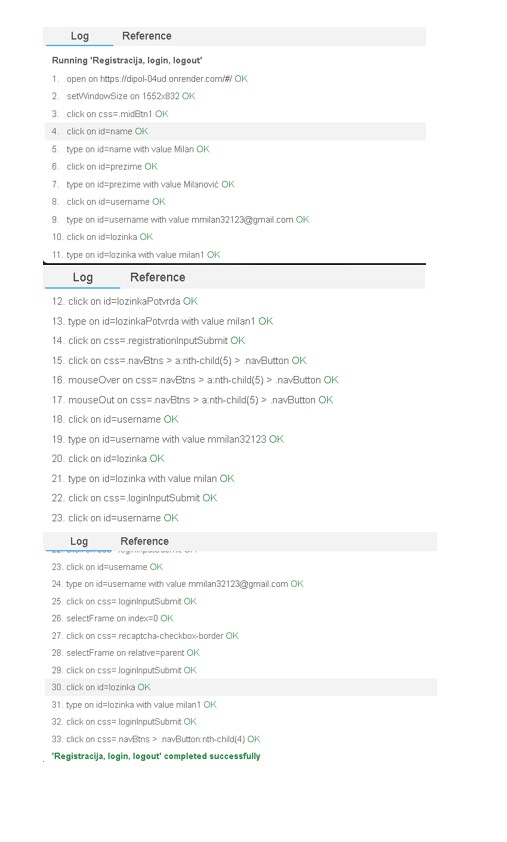
\includegraphics[width=8cm]{slike/test_1.jpg}
			 				\caption{test 1}
			 				\label{fig:fer-logo}
			 			\end{figure}
			 \end{itemize}
			 
			 \newpage
			 
			 \begin{itemize}
			 	\item Drugi slučaj - ulaz
			 	\begin{enumerate}
			 		\item Otvaranje stranice s konferencijama u web pregledniku
			 		\item Pritisćemo tipku "Pristupi" na nekoj od konferencija
			 		\item Unosimo pogrešnu lozinku za konferenciju
			 		\item Unosimo ispravnu lozinku za konferenciju
			 		\item Pritišćemo tipku "VOTE" za neki radi
			 		\item Pritišćemo tipku "VOTE" za neki drugi rad
			 	\end{enumerate}
			 	\item Drugi slučaj - očekivani rezultati
			 	\begin{enumerate}
			 		\item Prikazuju se sve aktivne i nadolazeće konferencije te vremenska prognoza za aktivne konferencije
			 		\item Prikazuje nam se polje za upis lozinke za konferenciju
			 		\item Iskače skočni prozor koji nam govori da lozinka nije ispravna
			 		\item Ulazimo u konferenciju gdje nam se prikazuju radovi
			 		\item Glasamo za taj rad, te sada na tipci piše "VOTED"
			 		\item Ništa se ne dogodi jer nam nije dopušteno glasati za više od jednog rada
			 	\end{enumerate}
			 	\item Prikaz rezultata
			 	\begin{figure}[htb]
			 		\centering
			 		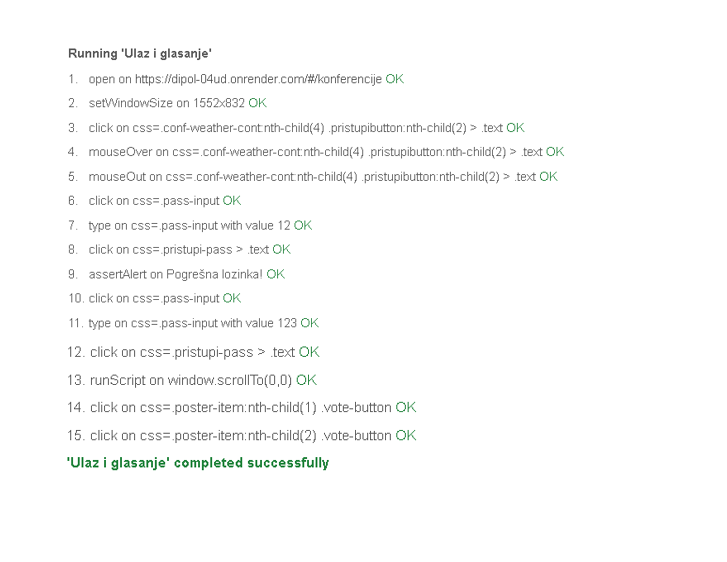
\includegraphics[width=11cm]{slike/test_2.png}
			 		\caption{test 2}
			 		\label{fig:fer-logo}
			 	\end{figure}
			 \end{itemize}
			 
			 \newpage
			 
			 \begin{itemize}
			 	\item Treći slučaj - ulaz
			 	\begin{enumerate}
			 		\item Otvaranje stranice za prošle konferencije u web pregledniku
			 		\item Pritinemo tipku "Pregledaj rezultate"
			 		\item Pritinemo tipku "Galerija fotografija"
			 		\item Pritisnemo svaku fotografiju jednom
			 		\item Pritisnemo tipku "Preuzmi odabrane fotografije"
			 	\end{enumerate}
			 	\item Treći slučaj - očekivani rezultati
			 	\begin{enumerate}
			 		\item Prikazuju se sve prošle konferencije
			 		\item Otvara se stranica s rezultatime te konferencije
			 		\item Otvara se galerija sa svim slikama te konferencije
			 		\item Svaka fotografije se označuje (obrub mijenja boju)
			 		\item Svaka se fotografije preuzima lokalno na uređaj
			 	\end{enumerate}
			 	\item Prikaz rezultata
			 	\begin{figure}[htb]
			 		\centering
			 		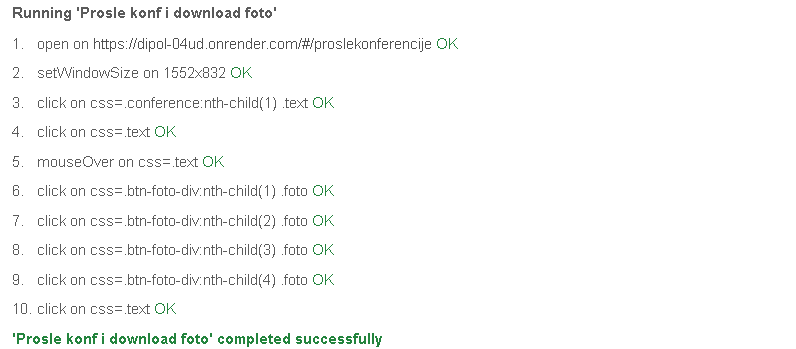
\includegraphics[width=11cm]{slike/test_3.png}
			 		\caption{test 3}
			 		\label{fig:fer-logo}
			 	\end{figure}
			 \end{itemize}
			 
			 \newpage
			 
			 \begin{itemize}
			 	\item Četvrti slučaj - ulaz
			 	\begin{enumerate}
			 		\item Otvaranje stranice s konferencijama u web pregledniku
			 		\item Pritisnemo tipku "Dodaj konferenciju"
			 		\item Pritisnemo tipku "Unesi" bez da unesemo sve podatke
			 		\item Pritisnemo tipku "Unesi" nakon što smo unijeli sve podatke, ali nismo u potpunosti unijeli datum ili vrijeme
			 		\item Pritisnemo tipku "Unesi" nakon što smo unijeli sve podatke, svi podaci su točni i potpuni
			 	\end{enumerate}
			 	\item Četvrti slučaj - očekivani rezultati
			 	\begin{enumerate}
			 		\item Prikazuju se sve aktivne i nadolazeće konferencije te vremenska prognoza za aktivne konferencije
			 		\item Otvara se stranica za dodavanje konferencije
			 		\item Pojavljuje se napomena da ispunimo prvo po redu polje koje nije ispunjeno
			 		\item Pojavljuje se napomena kod polja za datum ili vrijeme koja glasi "Unesite važeću vrijednost. Ovo je polje nepotpuno ili sadrži nevažeći datum."
			 		\item Vraćamo se na stranicu s konferencijama te ako smo unijeli datum koji je već prošao, konferencija se prikazuje na stranici "Prošle konferencije"
			 		\item Vraćamo se na stranicu s konferencijama te ako smo unijeli tek nadolazeći datum, konferencija se prikazuje na stranici "Konferencije" pod "Nadolazeće konferencije"
			 		\item Vraćamo se na stranicu s konferencijama te ako smo unijeli datum početka prije trenutnog vremena, a datum završetka nakon trenutnog vremena, konferencija se prikazuje na stranici "Konferencije" pod "Aktivne konferencije"
			 	\end{enumerate}
			 	\item Prikaz rezultata
			 	\begin{figure}[htb]
			 		\centering
			 		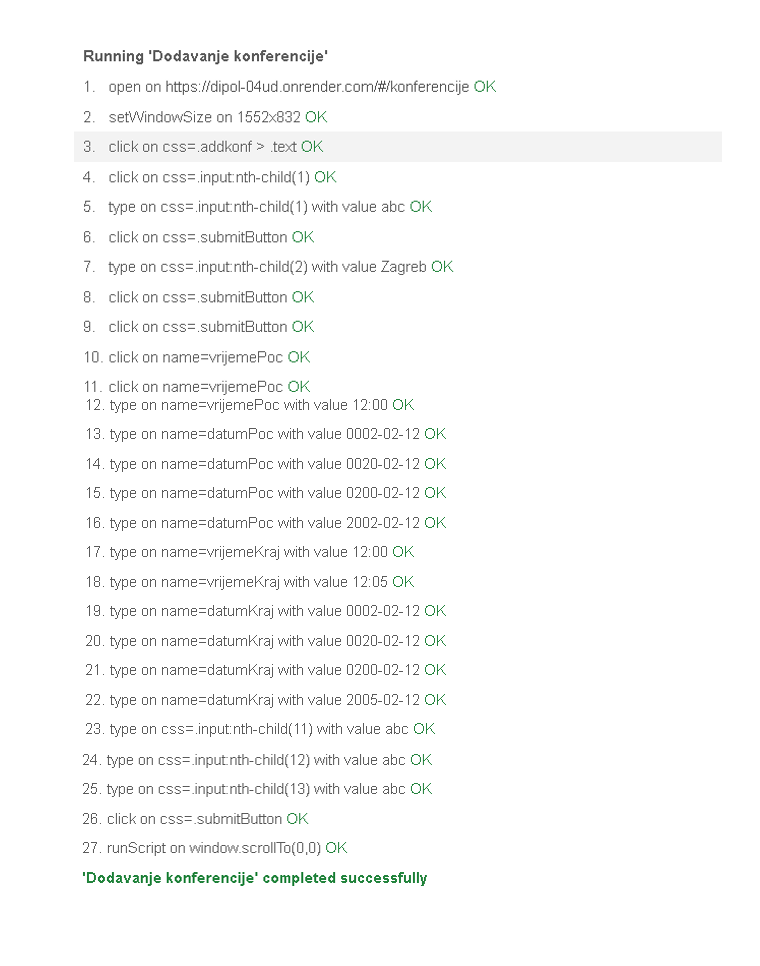
\includegraphics[width=11cm]{slike/test_4.png}
			 		\caption{test 4}
			 		\label{fig:fer-logo}
			 	\end{figure}
			 \end{itemize}
			 
			 \newpage
			 \newpage
			 
			 \begin{itemize}
			 	\item Peti slučaj - ulaz
			 	\begin{enumerate}
			 		\item Otvaranje stranice s konferencijama u web pregledniku
			 		\item Pod nadolazećim konferencijama pritisnemo tipku "Dodaj voditelja"
			 		\item Pritisnemo tipku "Unesi" bez da upišemo "Mail voditelja"
			 		\item Pritisnemo tipku "Unesi" s neispravno ispunjenim poljem "Mail voditelja"
			 		\item Pritisnemo tipku "Unesi" s ispravno ispunjenim poljem "Mail voditelja", ali ta e-mail adresa se ne nalazi u bazi podataka
			 		\item Pritisnemo tipku "Unesi" s ispravno ispunjenim poljem "Mail voditelja" i ta e-mail adresa se nalazi u bazi podataka
			 	\end{enumerate}
			 	\item Peti slučaj - očekivani rezultati
			 	\begin{enumerate}
			 		\item Prikazuju se sve aktivne i nadolazeće konferencije te vremenska prognoza za aktivne konferencije
			 		\item Otvara se stranica za dodavanje voditelja
			 		\item Pojavljuje se napomena "Ispunite ovo polje" (polje "Mail voditelja")
			 		\item Pojavljuje se napomena "Uključite znak @ u e-adresu."
			 		\item Javlja se greška "E-mail nije pronađen"
			 		\item Vraćamo se na stranicu s konferencijama
			 	\end{enumerate}
			 	\item Prikaz rezultata
			 	\begin{figure}[htb]
			 		\centering
			 		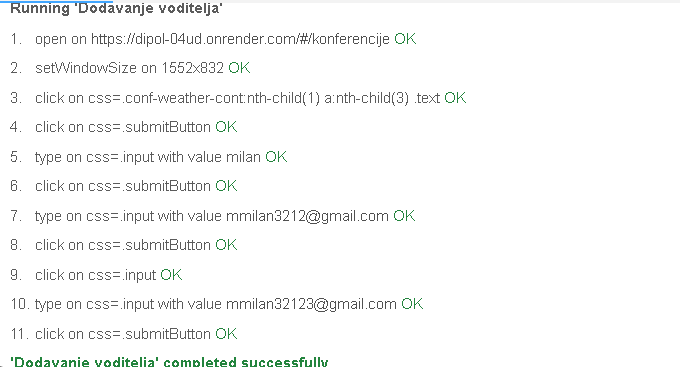
\includegraphics[width=11cm]{slike/test_5.png}
			 		\caption{test 5}
			 		\label{fig:fer-logo}
			 	\end{figure}
			 \end{itemize}
			 
			 	
			 	
			\eject 
		
		
		\section{Dijagram razmještaja}
			

			
			 \textit{}Dijagram razmještaja predstavlja strukturalni UML dijagram koji opisuje organizaciju sustava, fokusirajući se na međuodnos hardverskih i softverskih dijelova. Ključni elementi dijagrama uključuju čvorove, artefakte i poveznice. Čvorovi reprezentiraju stvarne uređaje (označeni stereotipom "device") ili izvođenja okoline (označena stereotipom "execution environment"), kao što su operativni sustav, virtualni strojevi na različitim razinama i slično. Artefakt predstavlja konkretnu realizaciju programske komponente, poput datoteka s izvornim ili izvršnim kodom, tablica u bazama podataka, skripti itd. Ovisnosti na dijagramu ilustriraju odnose među različitim artefaktima.
			 
			 Naš sustav temelji se na arhitekturi "klijent-poslužitelj", gdje se komunikacija između računala korisnika i računala poslužitelja odvija putem HTTP veze. Na računalu poslužitelja smješteni su web poslužitelj i poslužitelj baze podataka. Klijent, koristeći web preglednik, pristupa web aplikaciji.
			 
			 \begin{figure}[htb]
			 	\centering
			 	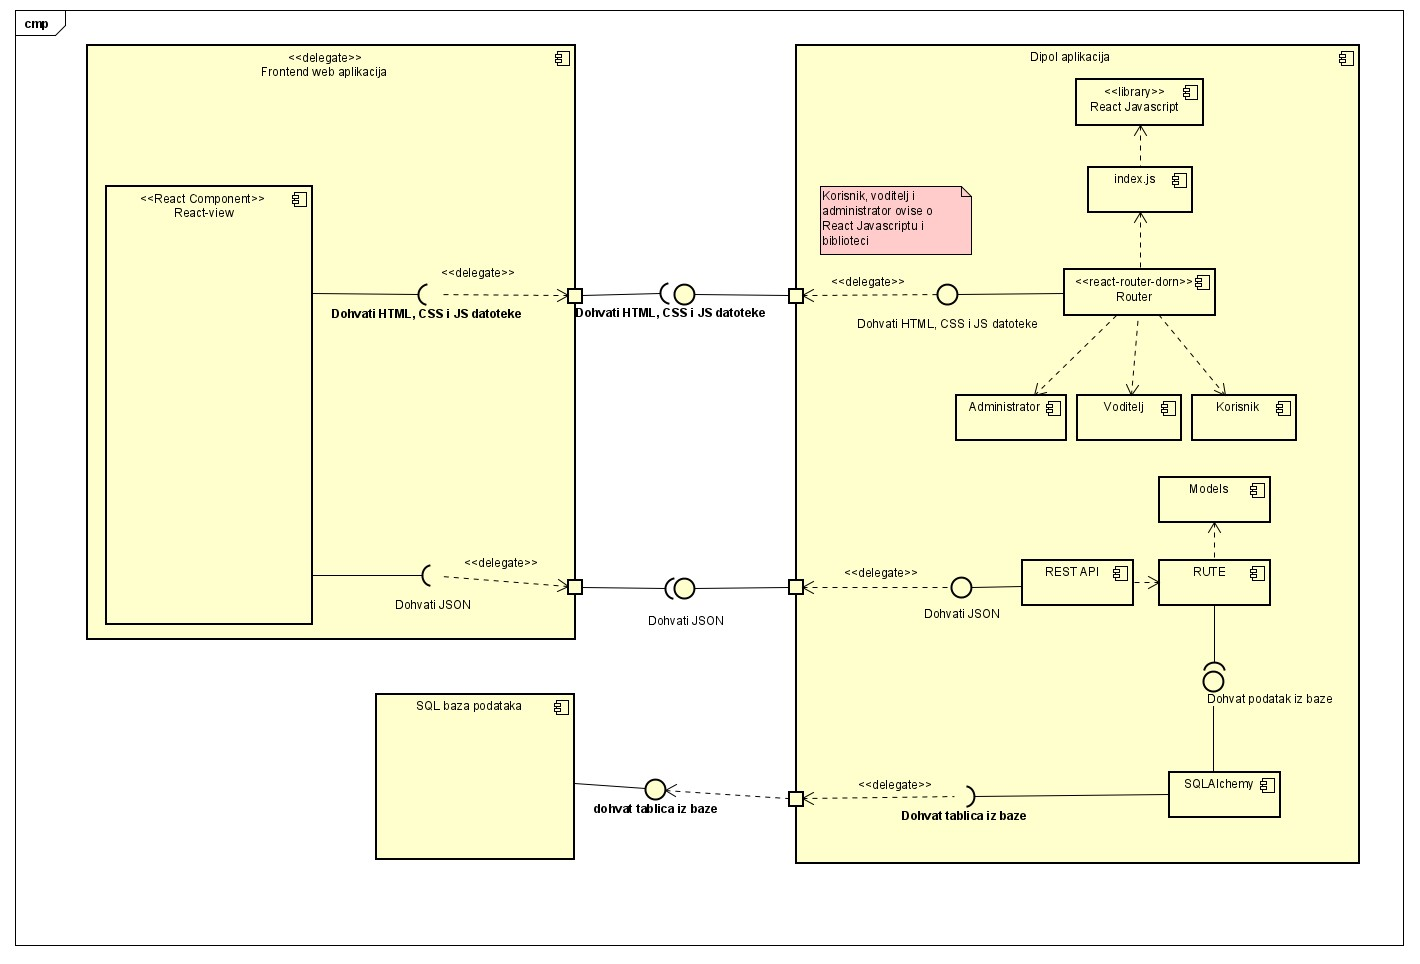
\includegraphics[width=11cm]{slike/Dijagram_komponensti.jpg}
			 	\caption{Dijagram razmještaja}
			 	\label{fig:fer-logo}
			 \end{figure}
			
			\eject 
		
		\section{Upute za puštanje u pogon}
		
			 \textit{}Aplikacija je puštena u pogon na javno dostupnom poslužitelju korištenjem besplatne usluge Render
			 
			 \subsection{Kreiranje baze podataka}
			 
			 	\text{} Baza podataka koju smo implementirali u aktivnoj verziji aplikacije je PostgreSQL, dok smo tijekom razvoja koristili pgAdmin bazu podataka. Na kontrolnoj ploči sustava Render, prilikom stvaranja nove baze podataka, odabiremo opciju PostgreSQL. Nakon toga, postavljamo naziv baze na "progi\textunderscore sri5", korisničko ime na "progi\textunderscore sri5\textunderscore user", dok je lozinka automatski generirana. Lokacija servera, odnosno regija gdje se baza podataka nalazi, je Frankfurt. Usluga nam omogućuje korištenje 1 GB besplatnog prostora za pohranu podataka.\\
			 	
			 	
				\begin{figure}[htb]
					\centering
					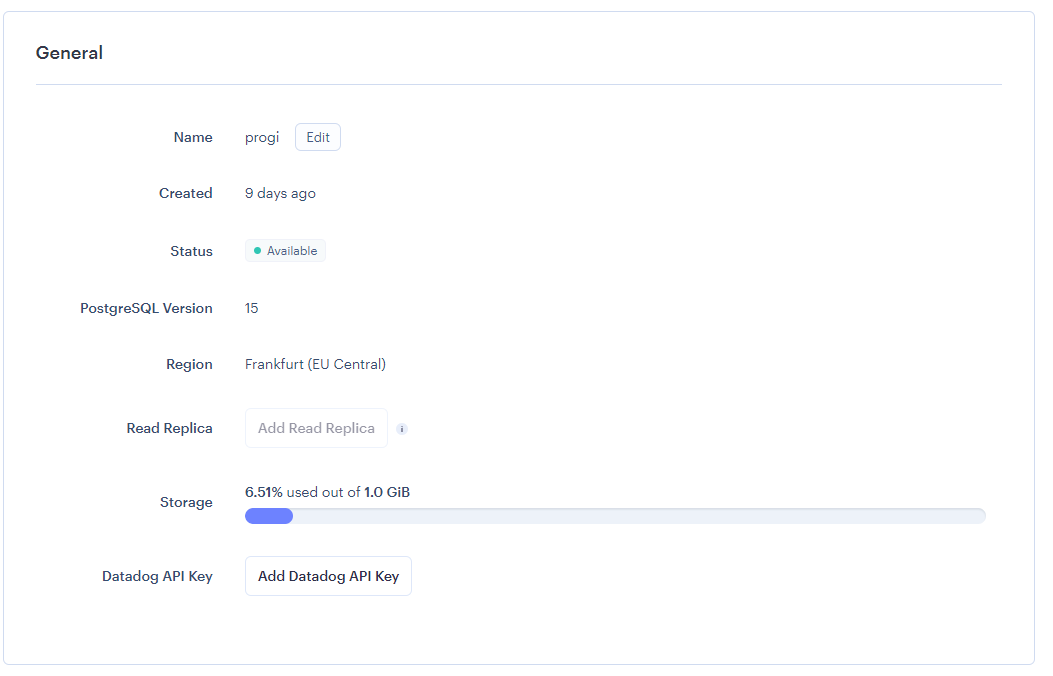
\includegraphics[width=15cm]{slike/baza_1.png}
					\caption{baza general}
					\label{fig:fer-logo}
				\end{figure}
				\newpage
				\begin{figure}[htb]
					\centering
					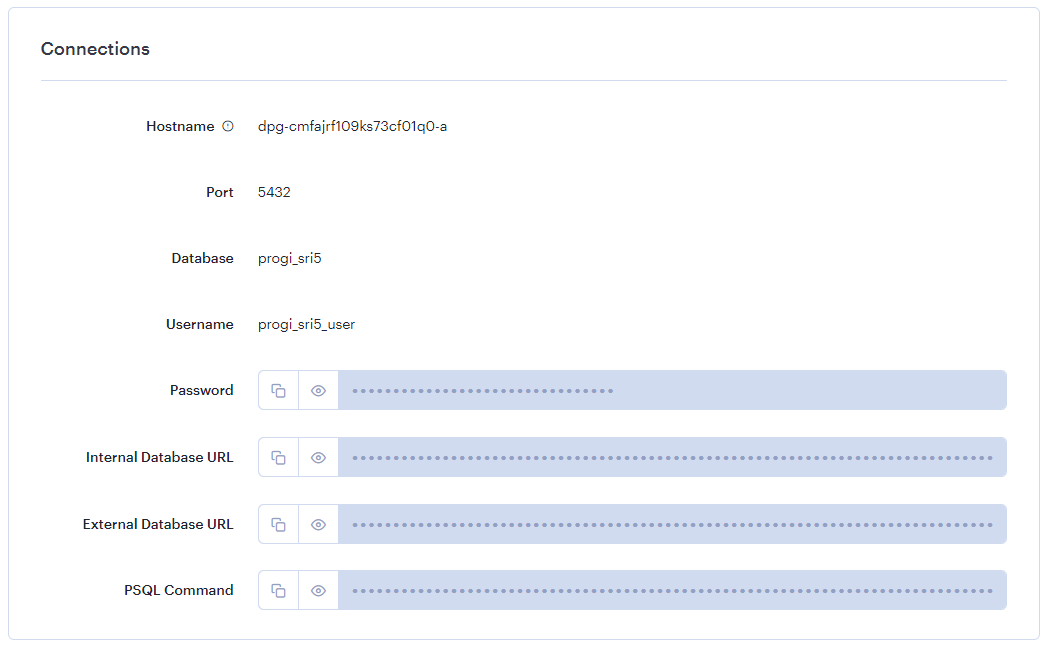
\includegraphics[width=15cm]{slike/baza_2.png}
					\caption{baza conection}
					\label{fig:fer-logo}
				\end{figure}
				
				\text{}Bazu podataka spajamo na pgAdmin V8 kako bi napravili potrebne tablice i atribute pomoću dobivenih podataka sa slike 5.8 te te podatke unosimo u prostor na slici 5.9 u pgAdmin nakon sto smo pritisnuli desni klin na "servers" -> "Register" -> "server".
				\newpage
				\begin{figure}[htb]
					\centering
					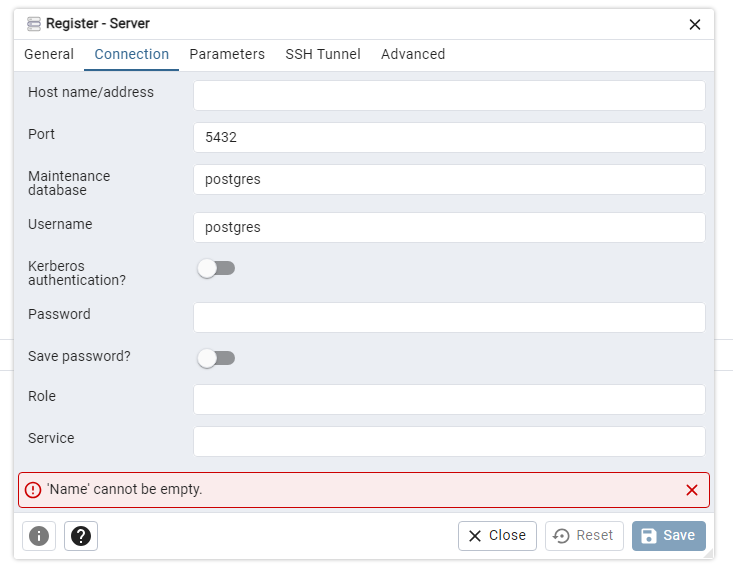
\includegraphics[width=15cm]{slike/server.png}
					\caption{Povezivanje baze na renderu}
					\label{fig:fer-logo}
				\end{figure}
				
			\subsection{Puštanje backend-a u pogon}
			
				\text{} Backend pustamo u pogon isto kao i bazu podataka na renderu. Pri pustanju Backenda u pogon na renderu prvo odabiremo gumb "New +" prikazan gore desno na priloženoj slici\\
			
			
				\begin{figure}[htb]
					\centering
					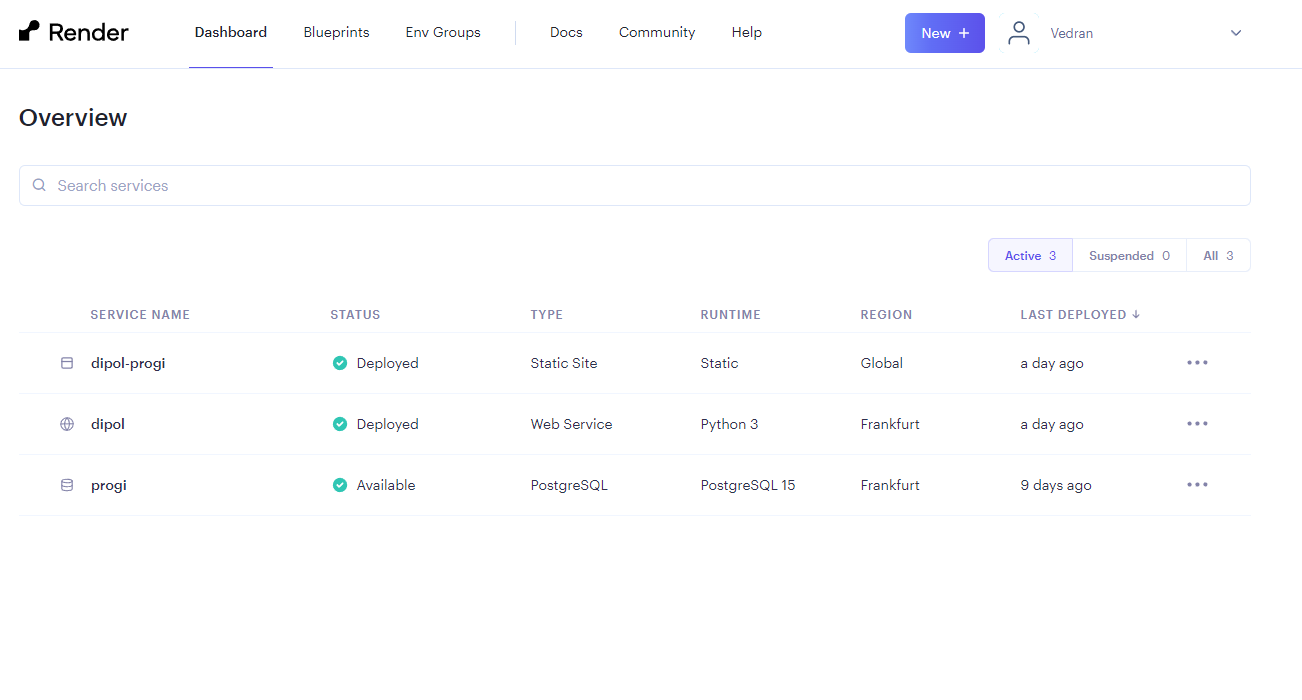
\includegraphics[width=15cm]{slike/back_1.png}
					\label{fig:fer-logo}
				\end{figure}
				\newpage
				\text{}Nakon toga odaibiremo opciju "Web service".\\
				
				\begin{figure}[htb]
					\centering
					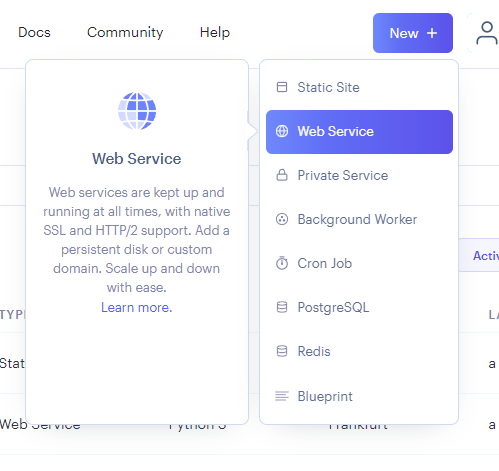
\includegraphics[width=10cm]{slike/back_2.png}
					\label{fig:fer-logo}
				\end{figure}
				\newpage
				\text{}Sada biramo kako je prikazanao na slici i pritišćemo gumb "Next".
				
				\begin{figure}[htb]
					\centering
					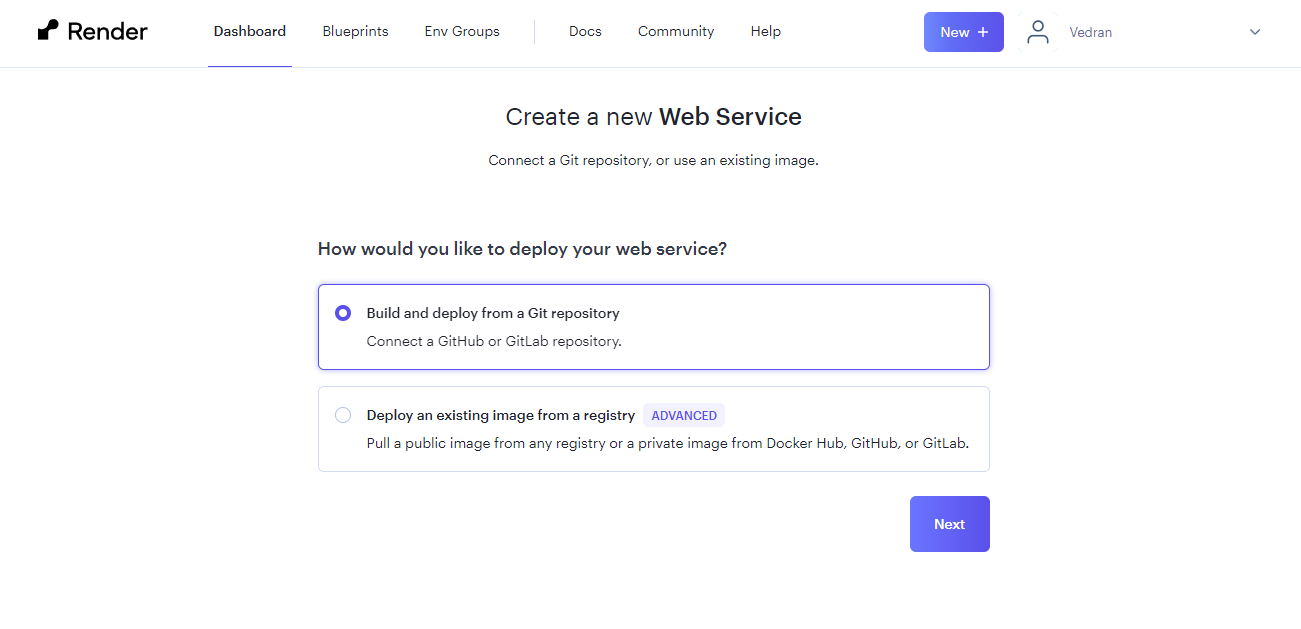
\includegraphics[width=15cm]{slike/back_3.png}
					\label{fig:fer-logo}
				\end{figure}
				\newpage
				\text{}Izabiremo server koji želimo pustiti u pogon te na stišćemo na njegov gumb "Connect".
				
				\begin{figure}[htb]
					\centering
					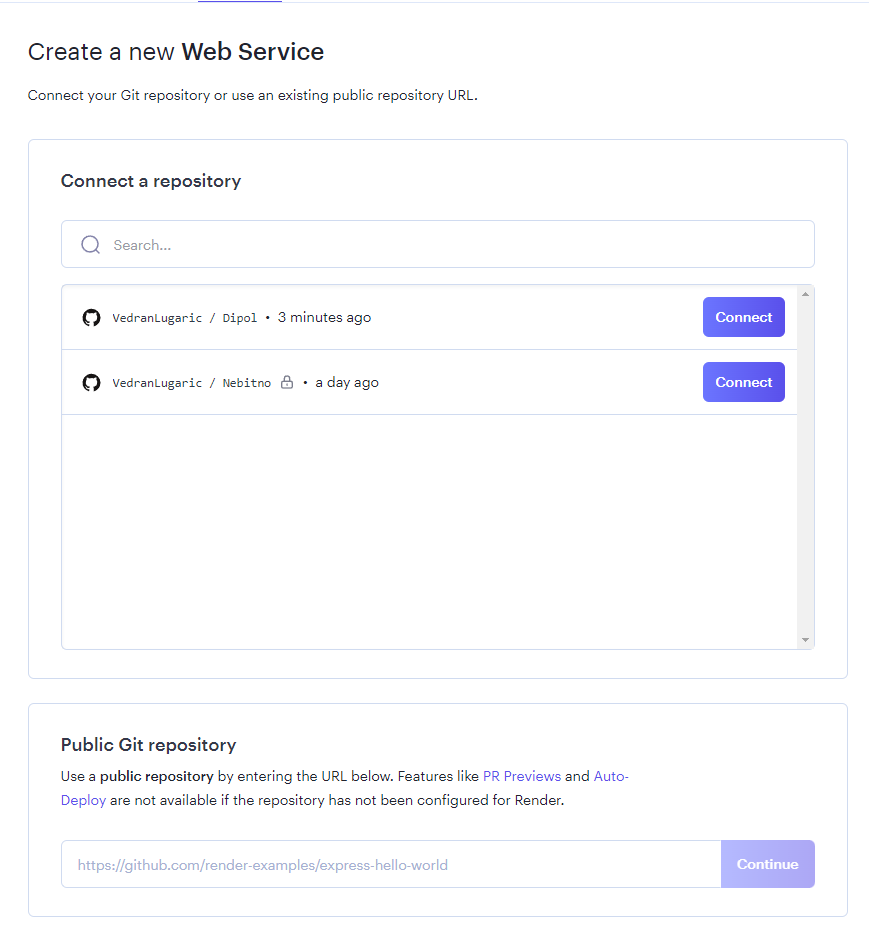
\includegraphics[width=15cm]{slike/back_4.png}
					\label{fig:fer-logo}
				\end{figure}
				\newpage
				\text{}Popunimo potrebna polja kako je prikazano na slici ispod i odabiremo besplatni plan (napomena: progi ključ se mora kopirati u polje desno od polja gdje piše progu ključ).
				
				\begin{figure}[htb]
					\centering
					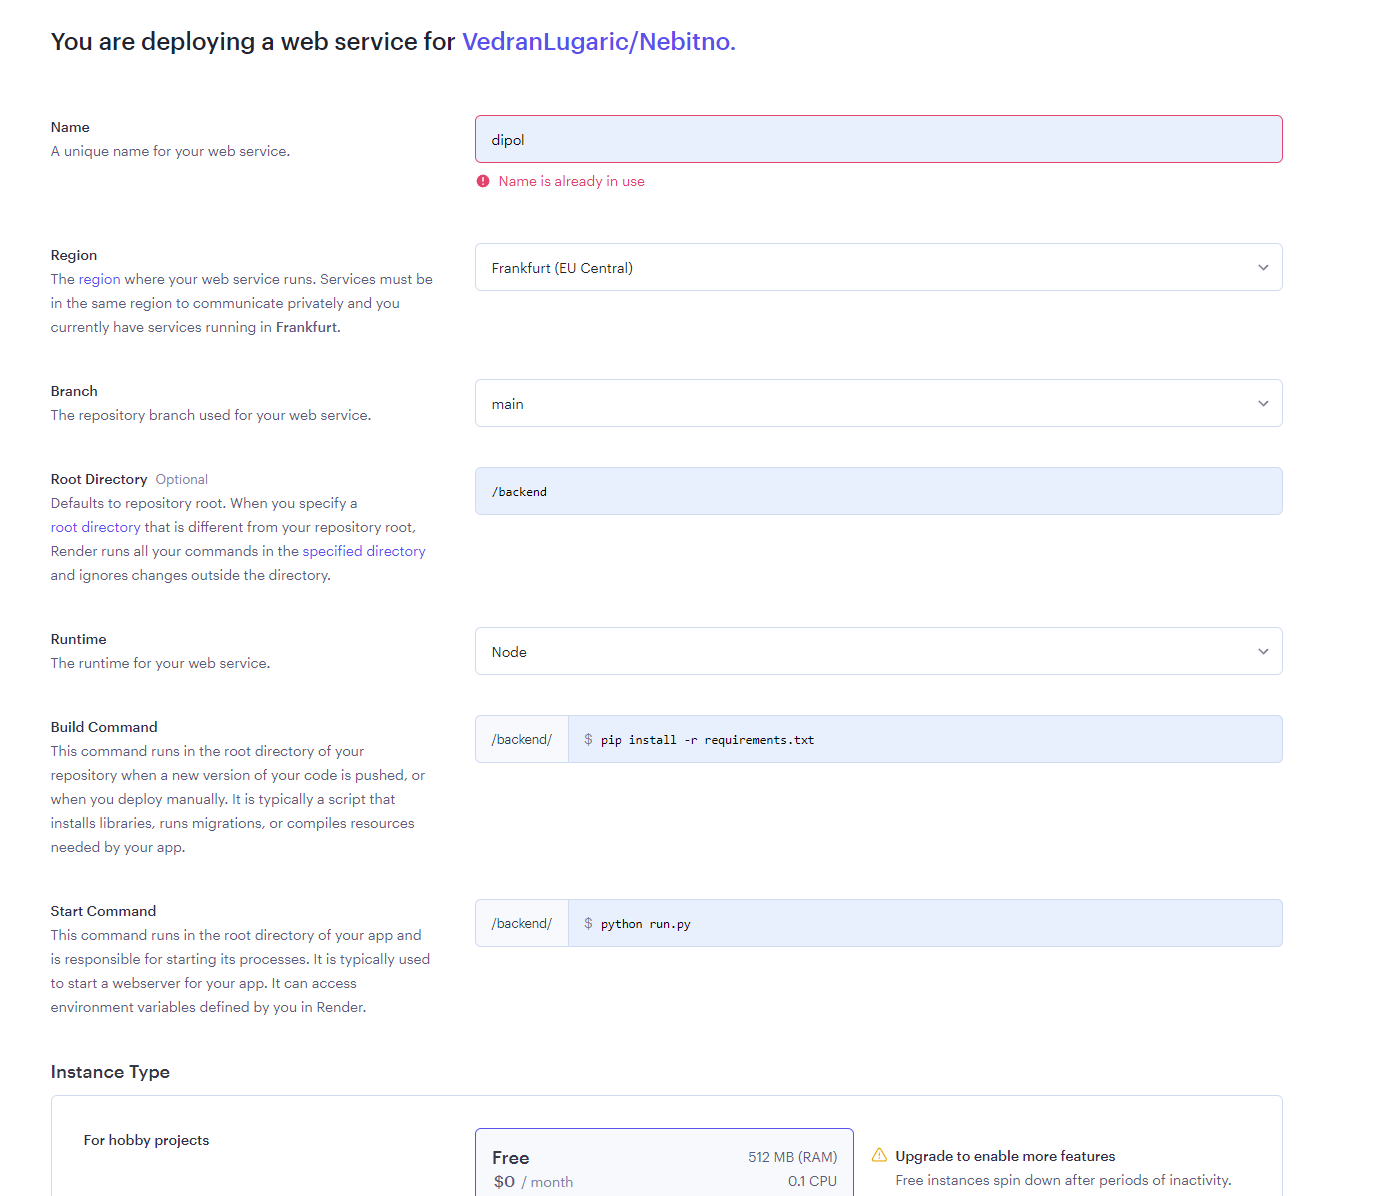
\includegraphics[width=15cm]{slike/back_5.png}
					\label{fig:fer-logo}
				\end{figure}
				\newpage
				\text{}Pritišćemo gumb "Create web service".
				
				\begin{figure}[htb]
					\centering
					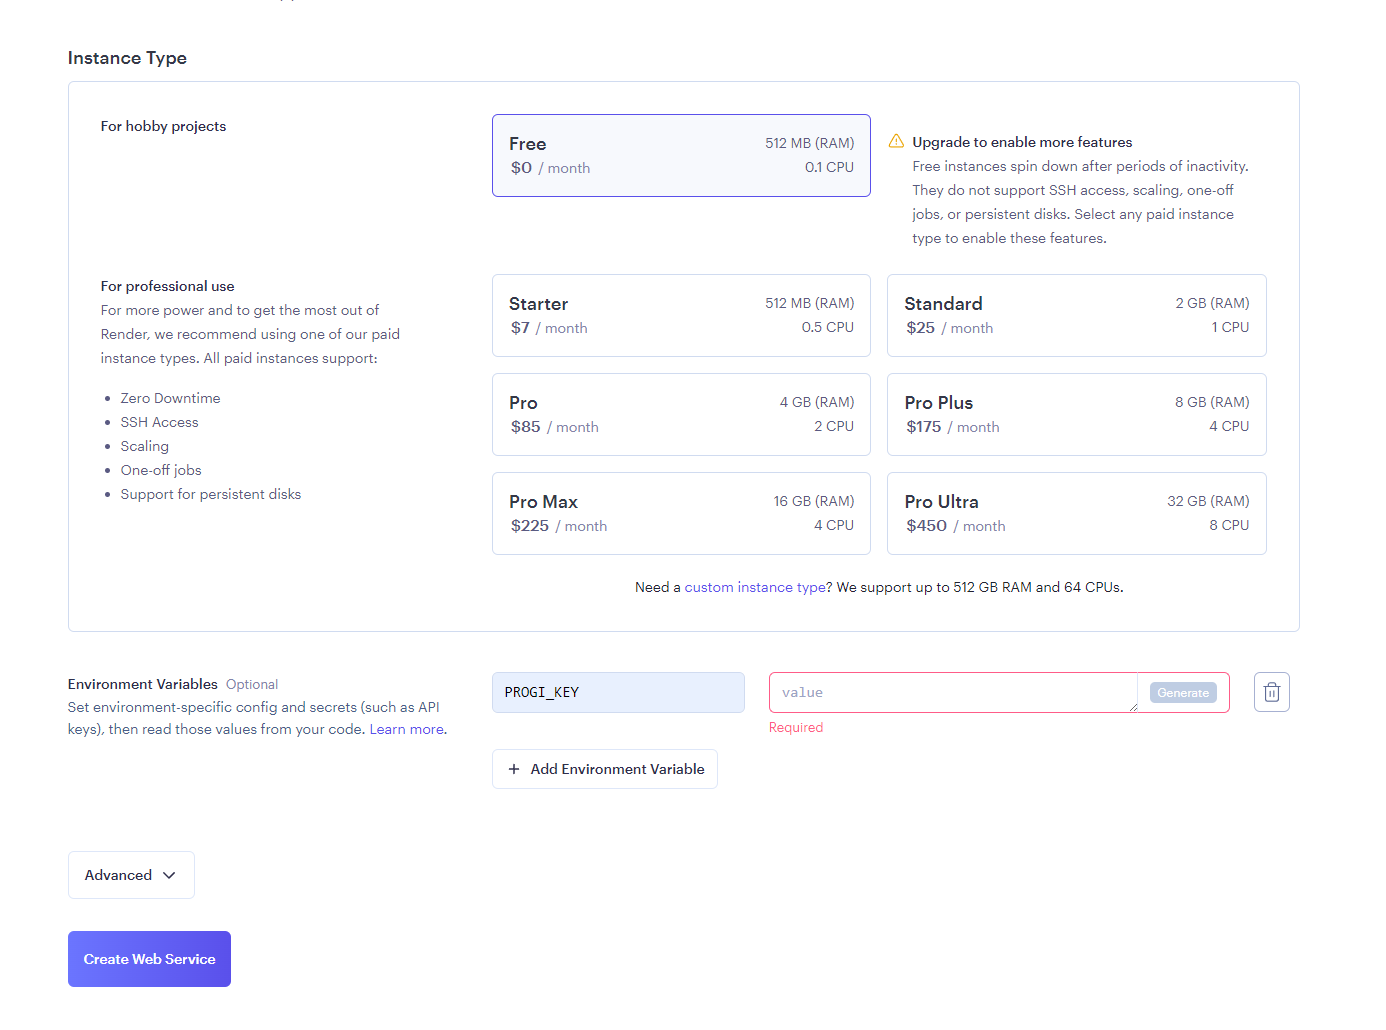
\includegraphics[width=15cm]{slike/back_6.png}
					\label{fig:fer-logo}
				\end{figure}
				\text{}Nakon provedenih svih radnji backend stranice je uspješno pušten u pogon.
			\subsection{Puštanje frontend-a u pogon}
			
				\text{} Frontend pustamo u pogon isto kao i bazu podataka na renderu. Pri pustanju Backenda u pogon na renderu prvo odabiremo gumb "New +" prikazan gore desno na priloženoj slici\\
				
				
				\begin{figure}[htb]
					\centering
					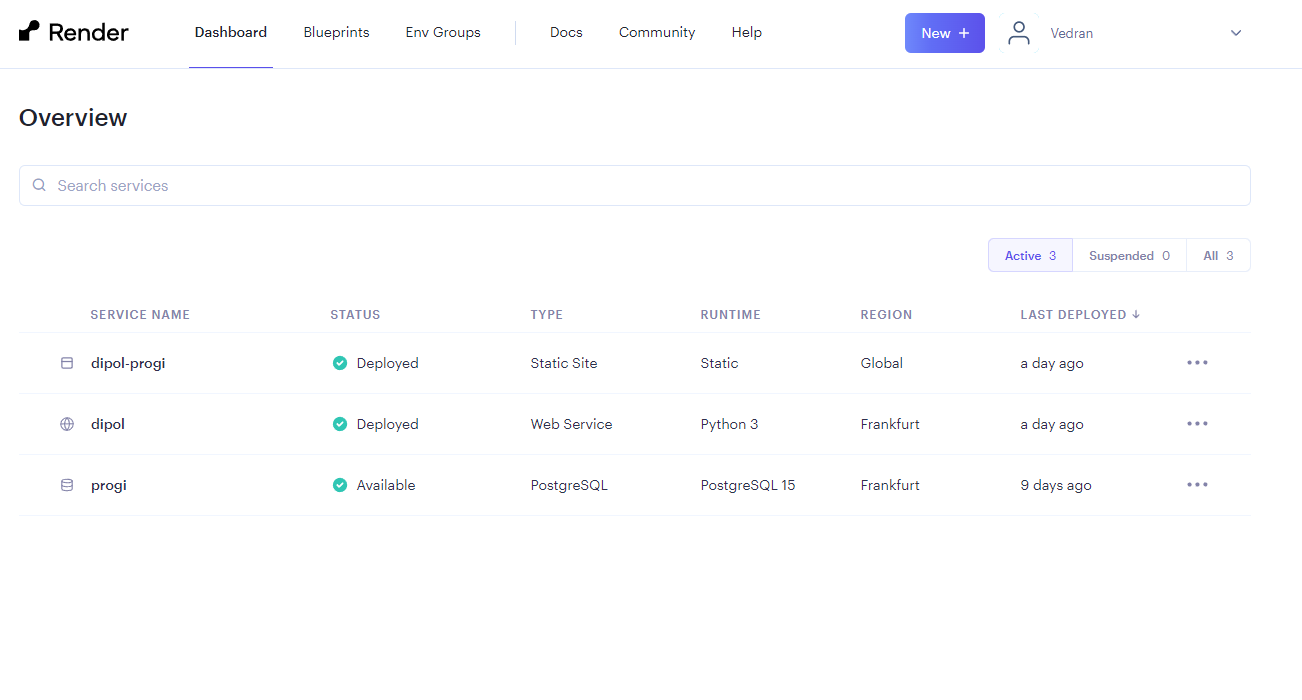
\includegraphics[width=15cm]{slike/back_1.png}
					\label{fig:fer-logo}
				\end{figure}
				\newpage
				\text{}Nakon toga odaibiremo opciju "Static Site".\\
				
				\begin{figure}[htb]
					\centering
					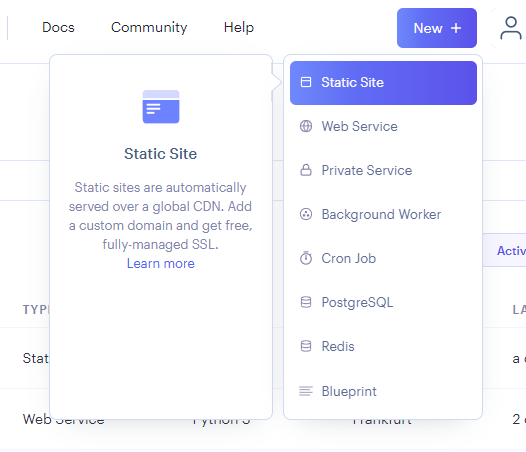
\includegraphics[width=10cm]{slike/front_2.png}
					\label{fig:fer-logo}
				\end{figure}
				\newpage
			
				\text{}Izabiremo server koji želimo pustiti u pogon te na stišćemo na njegov gumb "Connect".
				
				\begin{figure}[htb]
					\centering
					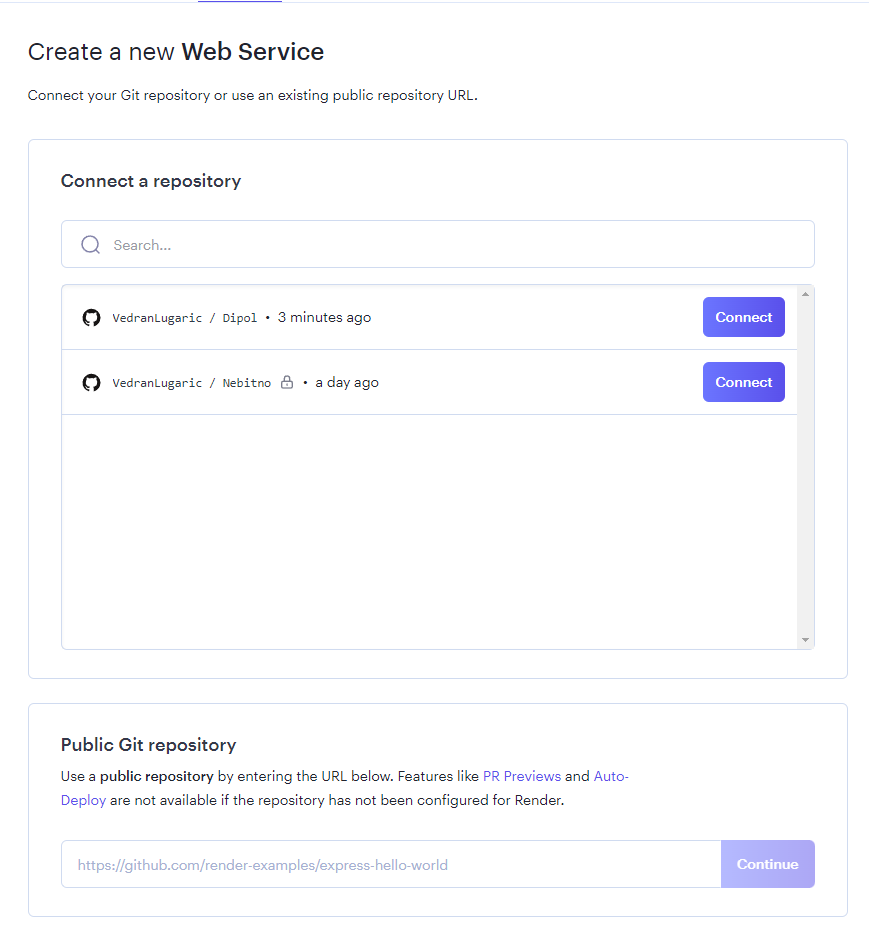
\includegraphics[width=15cm]{slike/back_4.png}
					\label{fig:fer-logo}
				\end{figure}
				\newpage
				\text{}Popunimo potrebna polja kako je prikazano na slici ispod .
				
				\begin{figure}[htb]
					\centering
					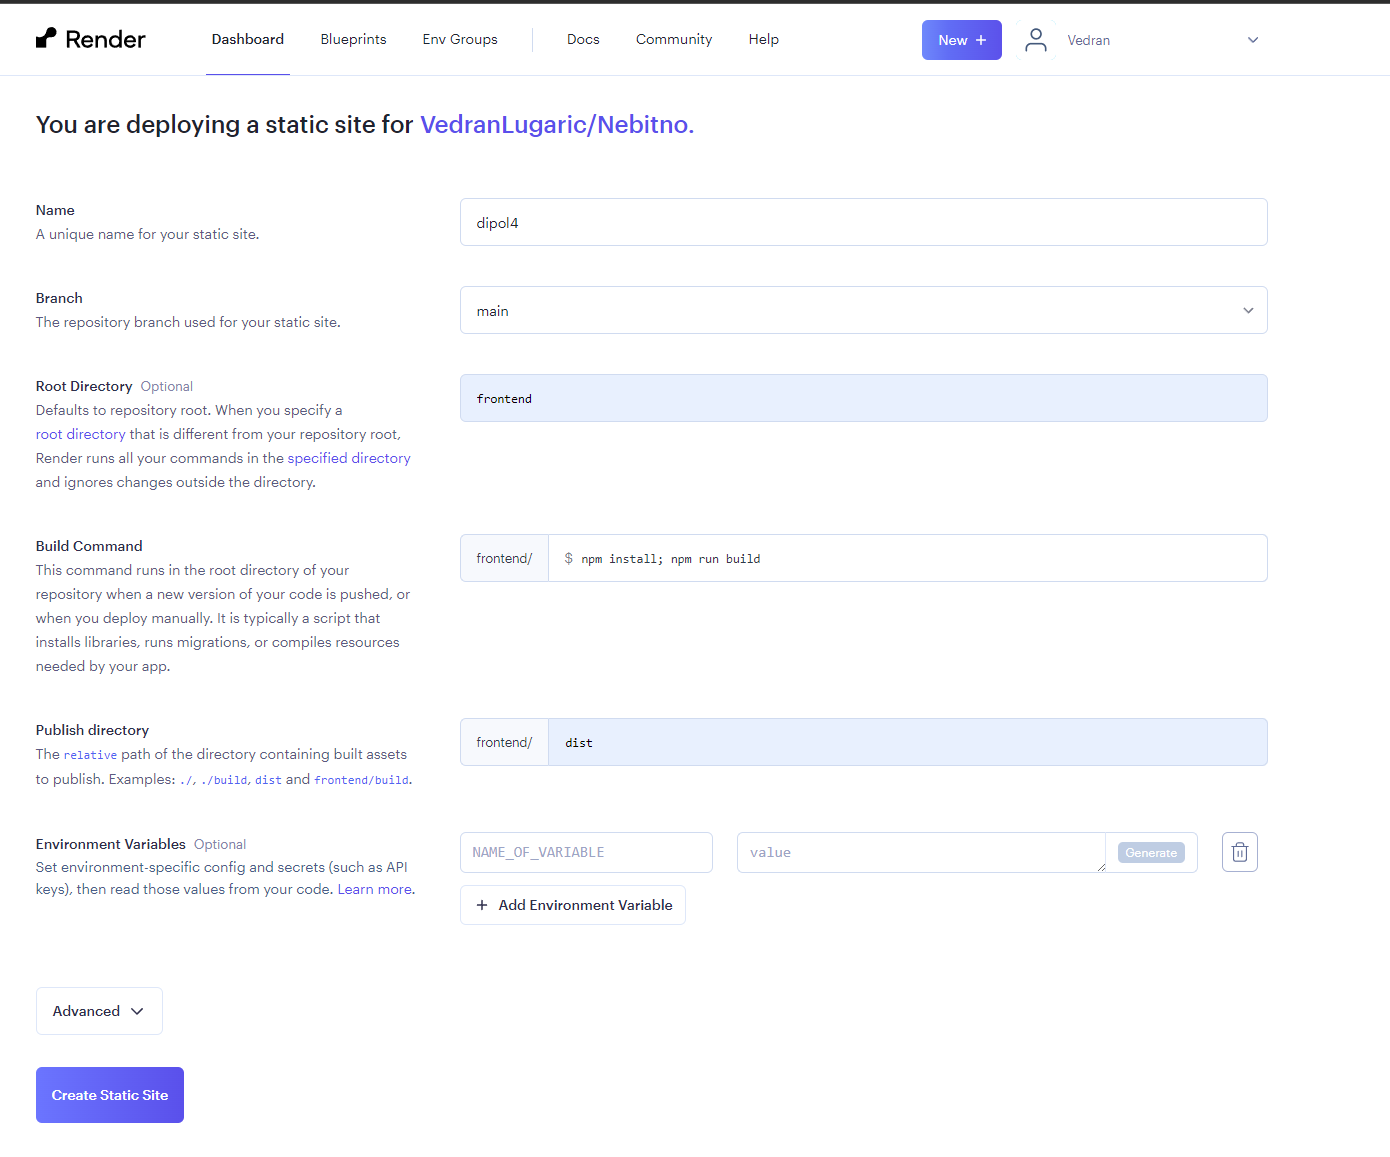
\includegraphics[width=15cm]{slike/front_3.png}
					\label{fig:fer-logo}
				\end{figure}
				
				\text{}Pritišćemo gumb "Create static site".
			
				\text{}Nakon provedenih svih radnji aplikacija je uspješno pušten u pogon.
			
			\eject 
	\chapter{Zaključak i budući rad}
		
		\textbf{\textit{dio 2. revizije}}\\
		
		 \textit{U ovom poglavlju potrebno je napisati osvrt na vrijeme izrade projektnog zadatka, koji su tehnički izazovi prepoznati, jesu li riješeni ili kako bi mogli biti riješeni, koja su znanja stečena pri izradi projekta, koja bi znanja bila posebno potrebna za brže i kvalitetnije ostvarenje projekta i koje bi bile perspektive za nastavak rada u projektnoj grupi.}
		
		 \textit{Potrebno je točno popisati funkcionalnosti koje nisu implementirane u ostvarenoj aplikaciji.}
		
		\eject 
	\chapter*{Popis literature}
		\addcontentsline{toc}{chapter}{Popis literature}
	 	
 		\textbf{\textit{Kontinuirano osvježavanje}}
	
		\textit{Popisati sve reference i literaturu koja je pomogla pri ostvarivanju projekta.}
		
		
		\begin{enumerate}
			
			
			\item  Programsko inženjerstvo, FER ZEMRIS, \url{http://www.fer.hr/predmet/proinz}
			
			\item  I. Sommerville, "Software engineering", 8th ed, Addison Wesley, 2007.
			
			\item  T.C.Lethbridge, R.Langaniere, "Object-Oriented Software Engineering", 2nd ed. McGraw-Hill, 2005.
			
			\item  I. Marsic, Software engineering book``, Department of Electrical and Computer Engineering, Rutgers University, \url{http://www.ece.rutgers.edu/~marsic/books/SE}
			
			\item  The Unified Modeling Language, \url{https://www.uml-diagrams.org/}
			
			\item  Astah Community, \url{http://astah.net/editions/uml-new}
		\end{enumerate}
		
		 
	
	
	\begingroup
	\renewcommand*\listfigurename{Indeks slika i dijagrama}
	%\renewcommand*\listtablename{Indeks tablica}
	%\let\clearpage\relax
	\listoffigures
	%\vspace{10mm}
	%\listoftables
	\endgroup
	\addcontentsline{toc}{chapter}{Indeks slika i dijagrama}


	
	\eject 
		
	\chapter*{Dodatak: Prikaz aktivnosti grupe}
		\addcontentsline{toc}{chapter}{Dodatak: Prikaz aktivnosti grupe}
		
		\section*{Dnevnik sastajanja}
		
		\textbf{\textit{Kontinuirano osvježavanje}}\\
		
		 \textit{U ovom dijelu potrebno je redovito osvježavati dnevnik sastajanja prema predlošku.}
		
		\begin{packed_enum}
			\item  sastanak
			
			\item[] \begin{packed_item}
				\item Datum: u ovom formatu: \today
				\item Prisustvovali: I.Prezime, I.Prezime
				\item Teme sastanka:
				\begin{packed_item}
					\item  opis prve teme
					\item  opis druge teme
				\end{packed_item}
			\end{packed_item}
			
			\item  sastanak
			\item[] \begin{packed_item}
				\item Datum: u ovom formatu: \today
				\item Prisustvovali: I.Prezime, I.Prezime
				\item Teme sastanka:
				\begin{packed_item}
					\item  opis prve teme
					\item  opis druge teme
				\end{packed_item}
			\end{packed_item}
			
			%
			
		\end{packed_enum}
		
		\eject
		\section*{Tablica aktivnosti}
		
			\textbf{\textit{Kontinuirano osvježavanje}}\\
			
			 \textit{Napomena: Doprinose u aktivnostima treba navesti u satima po članovima grupe po aktivnosti.}

			\begin{longtblr}[
					label=none,
				]{
					vlines,hlines,
					width = \textwidth,
					colspec={X[7, l]X[1, c]X[1, c]X[1, c]X[1, c]X[1, c]X[1, c]X[1, c]}, 
					vline{1} = {1}{text=\clap{}},
					hline{1} = {1}{text=\clap{}},
					rowhead = 1,
				} 
			
				\SetCell[c=1]{c}{} & \SetCell[c=1]{c}{\rotatebox{90}{\textbf{Ime Prezime voditelja}}} & \SetCell[c=1]{c}{\rotatebox{90}{\textbf{Ime Prezime }}} &	\SetCell[c=1]{c}{\rotatebox{90}{\textbf{Ime Prezime }}} & \SetCell[c=1]{c}{\rotatebox{90}{\textbf{Ime Prezime }}} &	\SetCell[c=1]{c}{\rotatebox{90}{\textbf{Ime Prezime }}} & \SetCell[c=1]{c}{\rotatebox{90}{\textbf{Ime Prezime }}} &	\SetCell[c=1]{c}{\rotatebox{90}{\textbf{Ime Prezime }}} \\  
				Upravljanje projektom 		&  &  &  &  &  &  & \\ 
				Opis projektnog zadatka 	&  &  &  &  &  &  & \\ 
				
				Funkcionalni zahtjevi       &  &  &  &  &  &  &  \\ 
				Opis pojedinih obrazaca 	&  &  &  &  &  &  &  \\ 
				Dijagram obrazaca 			&  &  &  &  &  &  &  \\ 
				Sekvencijski dijagrami 		&  &  &  &  &  &  &  \\ 
				Opis ostalih zahtjeva 		&  &  &  &  &  &  &  \\ 

				Arhitektura i dizajn sustava	 &  &  &  &  &  &  &  \\ 
				Baza podataka				&  &  &  &  &  &  &   \\ 
				Dijagram razreda 			&  &  &  &  &  &  &   \\ 
				Dijagram stanja				&  &  &  &  &  &  &  \\ 
				Dijagram aktivnosti 		&  &  &  &  &  &  &  \\ 
				Dijagram komponenti			&  &  &  &  &  &  &  \\ 
				Korištene tehnologije i alati 		&  &  &  &  &  &  &  \\ 
				Ispitivanje programskog rješenja 	&  &  &  &  &  &  &  \\ 
				Dijagram razmještaja			&  &  &  &  &  &  &  \\ 
				Upute za puštanje u pogon 		&  &  &  &  &  &  &  \\  
				Dnevnik sastajanja 			&  &  &  &  &  &  &  \\ 
				Zaključak i budući rad 		&  &  &  &  &  &  &  \\  
				Popis literature 			&  &  &  &  &  &  &  \\  
				&  &  &  &  &  &  &  \\ \hline 
				\textit{Dodatne stavke kako ste podijelili izradu aplikacije} 			&  &  &  &  &  &  &  \\ 
				\textit{npr. izrada početne stranice} 				&  &  &  &  &  &  &  \\  
				\textit{izrada baze podataka} 		 			&  &  &  &  &  &  & \\  
				\textit{spajanje s bazom podataka} 							&  &  &  &  &  &  &  \\ 
				\textit{back end} 							&  &  &  &  &  &  &  \\  
				 							&  &  &  &  &  &  &\\ 
			\end{longtblr}
					
					
		\eject
		\section*{Dijagrami pregleda promjena}
		
		\textbf{\textit{dio 2. revizije}}\\
		
		\textit{Prenijeti dijagram pregleda promjena nad datotekama projekta. Potrebno je na kraju projekta generirane grafove s gitlaba prenijeti u ovo poglavlje dokumentacije. Dijagrami za vlastiti projekt se mogu preuzeti s gitlab.com stranice, u izborniku Repository, pritiskom na stavku Contributors.}
		
	


\end{document} %naredbe i tekst nakon ove naredbe ne ulaze u izgrađen dokument 


